%!TEX root = ../thesis.tex
%*******************************************************************************
%****************************** Third Chapter **********************************
%*******************************************************************************
\chapter{Evaluation}

% **************************** Define Graphics Path **************************
\ifpdf
    \graphicspath{{07_Chapter6/Figs/Raster/}{07_Chapter6/Figs/PDF/}{07_Chapter6/Figs/}}
\else
    \graphicspath{{07_Chapter6/Figs/Vector/}{07_Chapter6/Figs/}}
\fi

\section{Evaluation Settings}

Appendix A presents a list of synthetic functions and real datasets that are used to evaluate the effectiveness of a Bayesian Optimization algorithm. 
I conduct experiments in the following settings as mentioned in chapter \ref{syntheticFunction}.
I must emphasize that I modified the algorithm of Tripathy et al., at is got stuck in local minima within the first five steps of algorithm 1.
For this, I set up the constraint that $\tau > 0$ (instead of $\tau \geq 0$). 
This allowed for small perturbations that kept on improving the loss.

\section{Quantitative evaluation}
To recapitulate, I will use log-likelihood, angle-difference measure and cumulative regret to compare the performance of different algorithms.
We present how the different algorithms perform on the regret measure using UCB as the acquisition function.
It is important to point out that all experiments capped the matrix identification step to about 30 minutes.
This is much less than in the original papers that we base the algorithm on.
The reason for this is that we want to have an acceptable comparison for medium-sized experiments, where time and computational resources can be restrictive (like on a users laptop). \\

I want to indicate whether the contribution of the performance comes from our subspace identification, or from the algorithm. 
For this, I start the discussion of every function with a plot that shows how the algorithm performs when the real subspace matrix $W_{\text{true}}$ is assumed to be found (Tripathy's algorithm is not applied; instead we return the $W_{\text{true}}$ instead of an approximated $\hat{W}$. \\

To keep the measurements fair across algorithms, I fix the noise variance of the GP and the kernel hyperparameters for each function. \\

I have multiple independent runs for each function.
However, as most of the runs show similar results, I display only one of them unless something is interesting to see.
The reader should notice that the individual runs do carry the same kernel parameters (unless an algorithm-specific function decides to change these).
This means that the algorithms should theoretically have similar properties as UCB on the vanilla function if the active subspace is identified or the dimensionality is effectively reduced. \\

In all of these graphs, we apply the subspace identification at the 100th timestep.
This means that we use the first 100 sampled points from UCB to identify a subspace.
Any other future projected point is projected onto this subspace before one optimization is taken.

Due to numerical errors recognized at later stages, the maximum dimension that I test over is 5.
When I set the real dimensionality of an environment (not the active dimensionality), the property $W^T \times W = I$ is violated.
Apart from that, all algorithms were implemented from scratch.
Any implemented gradients were unit-tested, and the respective analytical gradient was (successfully) compared with their numerical gradients.
To test the functionality of the subspace identification algorithm, I also wrote tests to make sure that the log-likelihood increases, and that some other properties presented in the respective paper are satisfied.

\subsection{Parabola}

The function to be learned and optimized over is the following:

\def\WParaboa2D{
\begin{bmatrix}
    0.500\\
    0.192
\end{bmatrix}}

\begin{equation}
f(x) = \left( \WParaboa2D^T x \right)^2
\end{equation}
where we have $x \in \mathbf{R}^2$ and $W \in \mathbf{R}^{2 \times 1}$.


\paragraph{Assume $\hat{W} = W_{\text{true}}$}: I present how the respective algorithms perform if we assume that Tripathy's Stiefel Manifold optimization finds the perfect matrix.
This measures how the algorithm performs when we assume perfect subspace identification.

\begin{figure}[H]
  \centering
      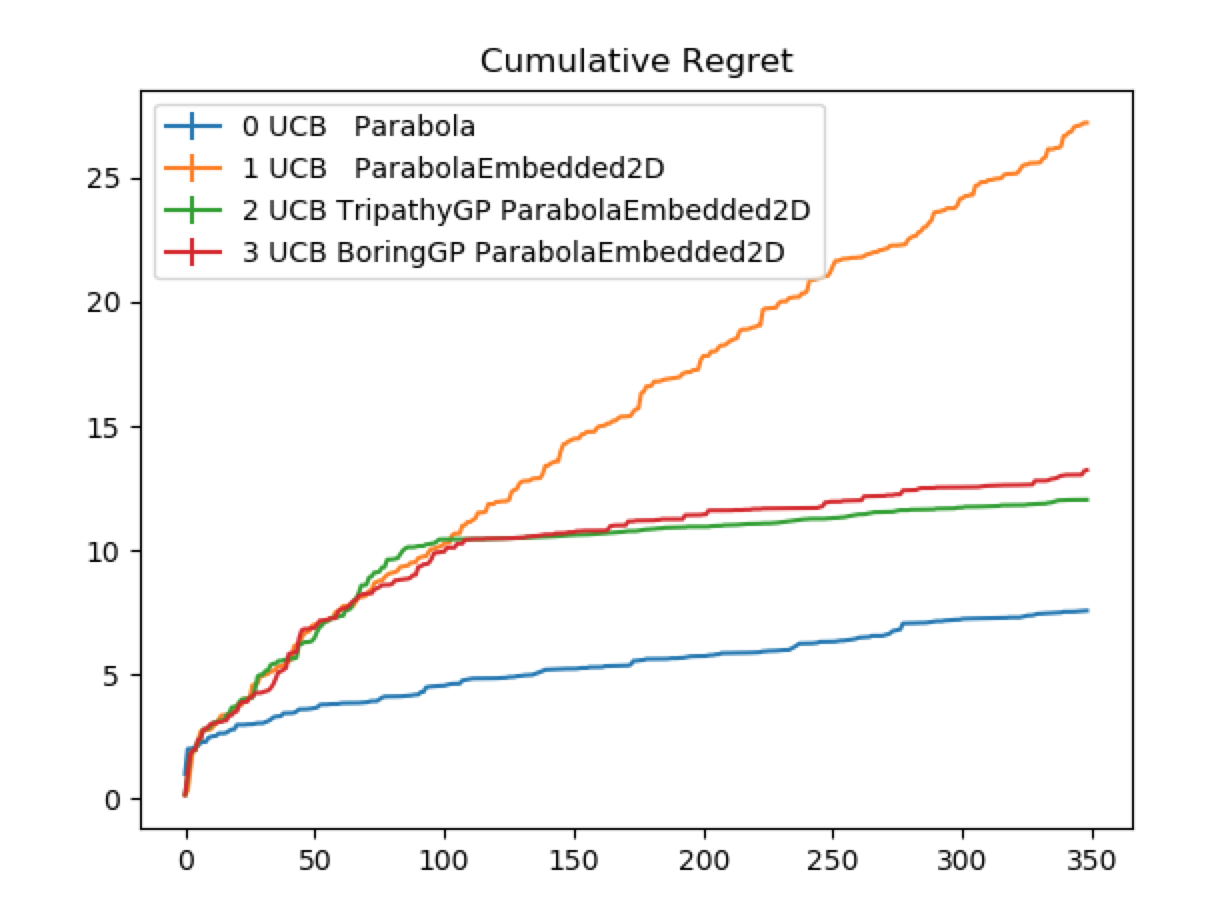
\includegraphics[width=0.5\textwidth]{reference_W_true/Parabola2D}
  \caption{UCB on a Parabola embedded in 2D space, when we assume that tripathy's method finds the real projection matrix.}
\end{figure}

\paragraph{Assume $\hat{W} \neq W_{\text{true}}$}: I now proceed with how different algorithms perform on the function described above.
This measures how the algorithm performs, when subspace identification is a part of the optimization process.

\begin{figure}[H]
  \centering
      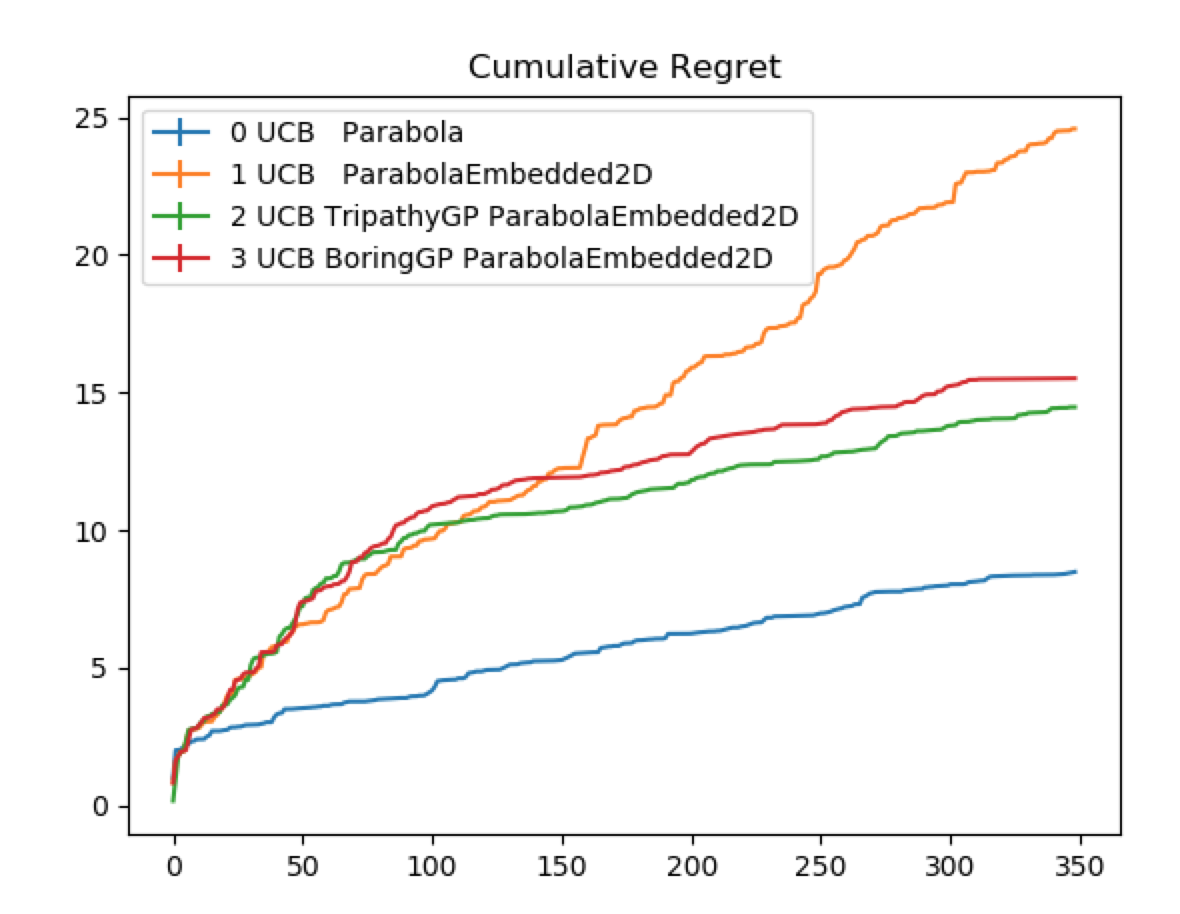
\includegraphics[width=0.5\textwidth]{W_hat_tripathy/Parabola2D_0}
  \caption{UCB on a Parabola embedded in 2D space.
  Tripathy's algorithm is applied to find a projection matrix $\hat{W}$.}
\end{figure}

One can easily see that the performance on UCB using Tripathy's matrix identification algorithm is similar to the case when we assume that Tripathy executes perfectly.


%One can see that REMBO without interleavings has very high variance amongst runs. 
%Sometimes it can find a suitable subspace (subfigure (c) and (d)), but on other runs, it fails to find an appropriate subspace.
%The reader should notice that most of these lines are linear.
%This may be the result of not tuning the hyperparameters during runs.
%In this case, the BORING algorithm assesses the same properties as the Tripathy model (as the number of passive dimensions is set to 0), with which the two models perform very similar on the regret curves. \\

\textbf{The log likelihood of the GP w.r.t the collected data points} of the Tripathy GP with the real matrix is comparable to the log-likelihood of the GP of the Tripathy model, where the active projection matrix is calculated using the algorithm (values of $-1.37$ and $-1.38$ or for a different run values of $195.32$ and $210.25$, where ranges are between  $-100$ and $700$).
One should notice, however, that the angle between the found matrix and the real projection matrix is almost always at $45°$ - a value that does not sound very intuitive, and for which the only reasonable explanation is that the optimization problem stays the same at this projection angle.
The reader can view graphs in a subsequent subsection.

\subsection{Camelback embedded in 3D}

The function to be learned and optimized over is the following:

\def\WCamelback3D{
\begin{bmatrix}
    -0.46554187 & -0.36224966 & 0.80749362 \\
     0.69737806 & -0.711918 & 0.08268378
\end{bmatrix}}

\begin{equation}
f(z_1, z_2) = \left( 4 - 2.1 * z_1^2 + \frac{z_1^4}{3} \right)  z_1^2 + z_1 *  z_2 + \left(-4 + 4 * z_2^2 \right) * z_2^2
\end{equation} \\

where we have $z = \left( \WCamelback3D^T x \right) $, and $ x \in \mathbf{R}^3$, $W \in \mathbf{R}^{2 \times 3}$ and where $z_1$ denotes the first entry of the $z$ vector, and $z_2$ denotes the second element of the $z$ vector.

\paragraph{Assume $\hat{W} = W_{\text{true}}$}: Again, I present how the respective algorithms perform if we assume that Tripathy's Stiefel Manifold optimization finds the perfect matrix.

\begin{figure}[H]
  \centering
      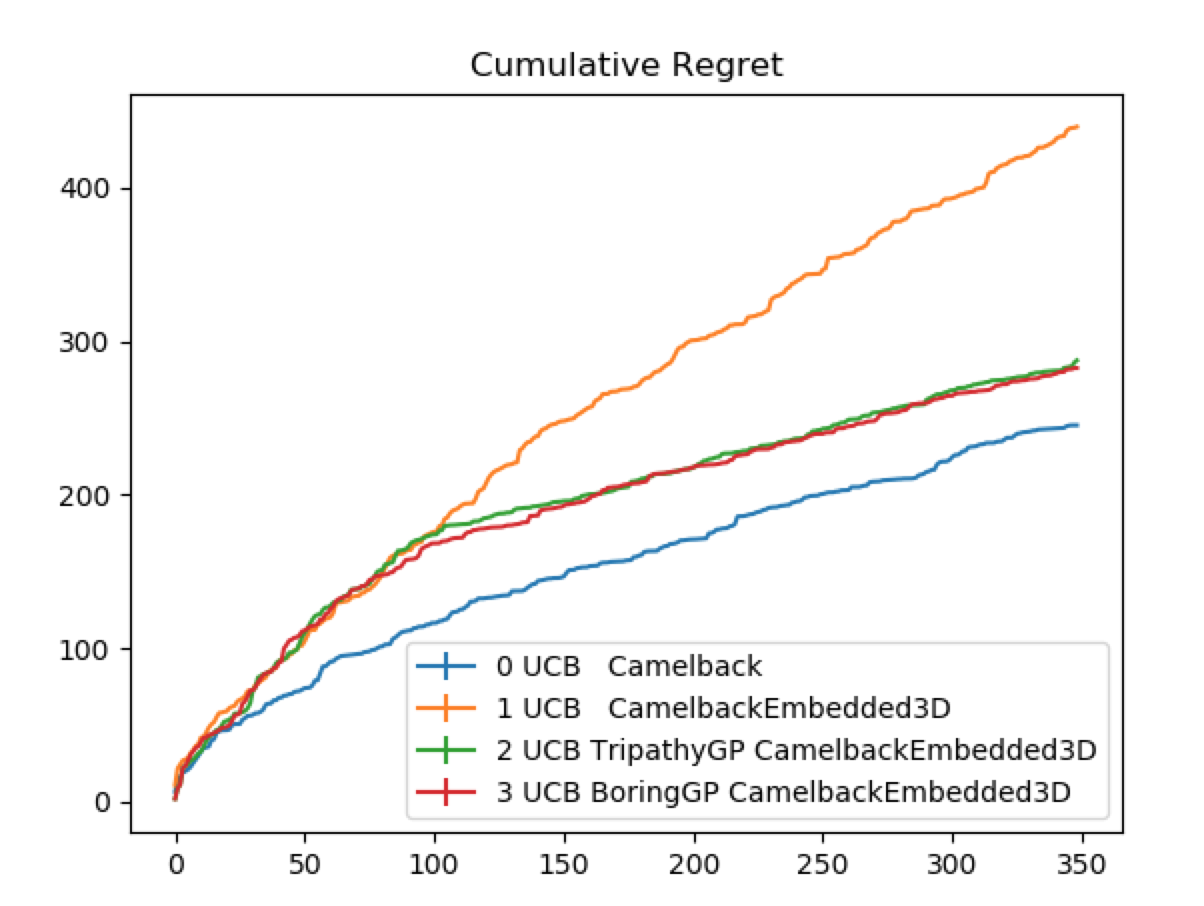
\includegraphics[width=0.5\textwidth]{reference_W_true/Camelback3D}
  \caption{UCB on a 2D Camelback function embedded in 3D space.
  This is when we assume that Tripathy finds the real projection matrix $W_{\text{true}}$}
\end{figure}

\paragraph{Assume $\hat{W} \neq W_{\text{true}}$}: Again, I now proceed with the performance, when the subspace identification is part of the optimization process.

\begin{figure}[H]
    \centering
    \begin{subfigure}[b]{0.40\textwidth}
        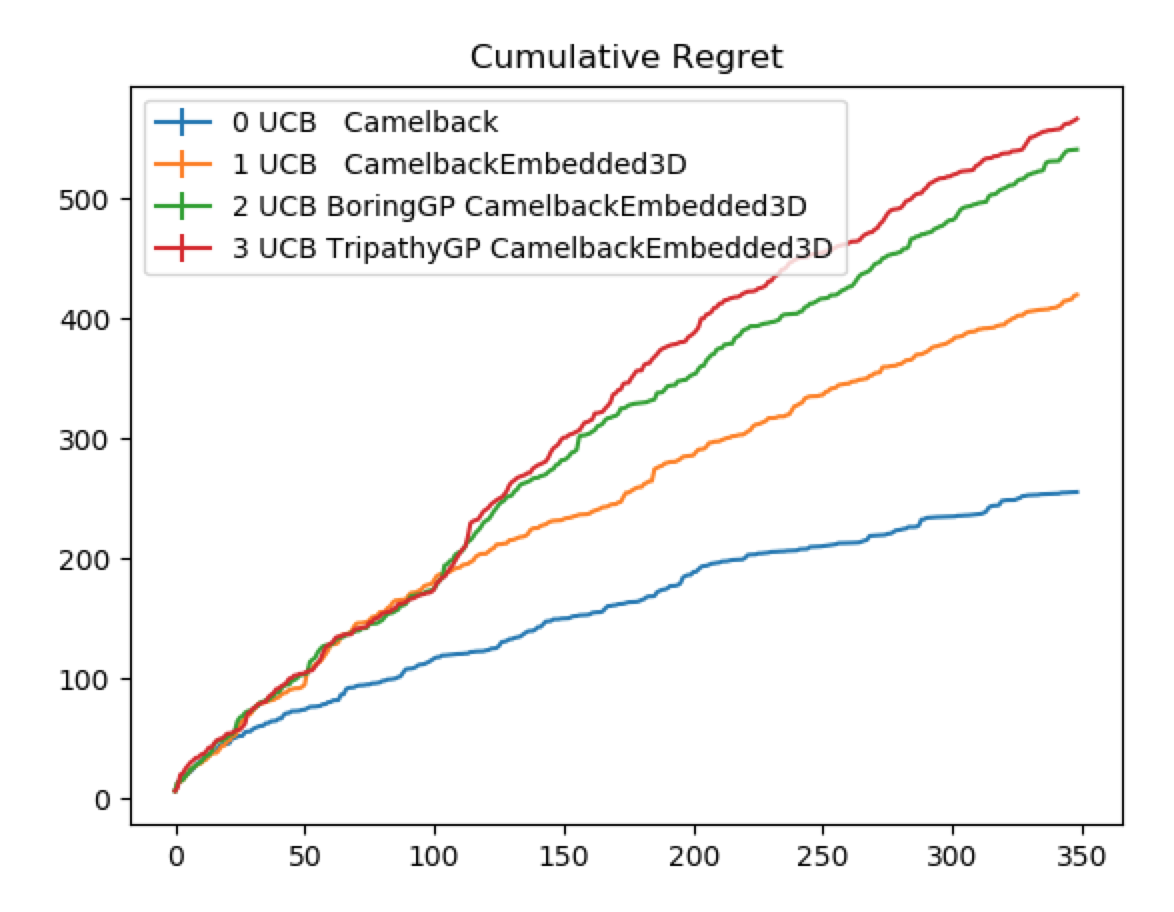
\includegraphics[width=\textwidth]{W_hat_tripathy/Camelback3D_0}
        \label{fig:gull}
        \caption{Run 1}
    \end{subfigure}
    %add desired spacing between images, e. g. ~, \quad, \qquad, \hfill etc. 
      %(or a blank line to force the subfigure onto a new line)
    \begin{subfigure}[b]{0.40\textwidth}
        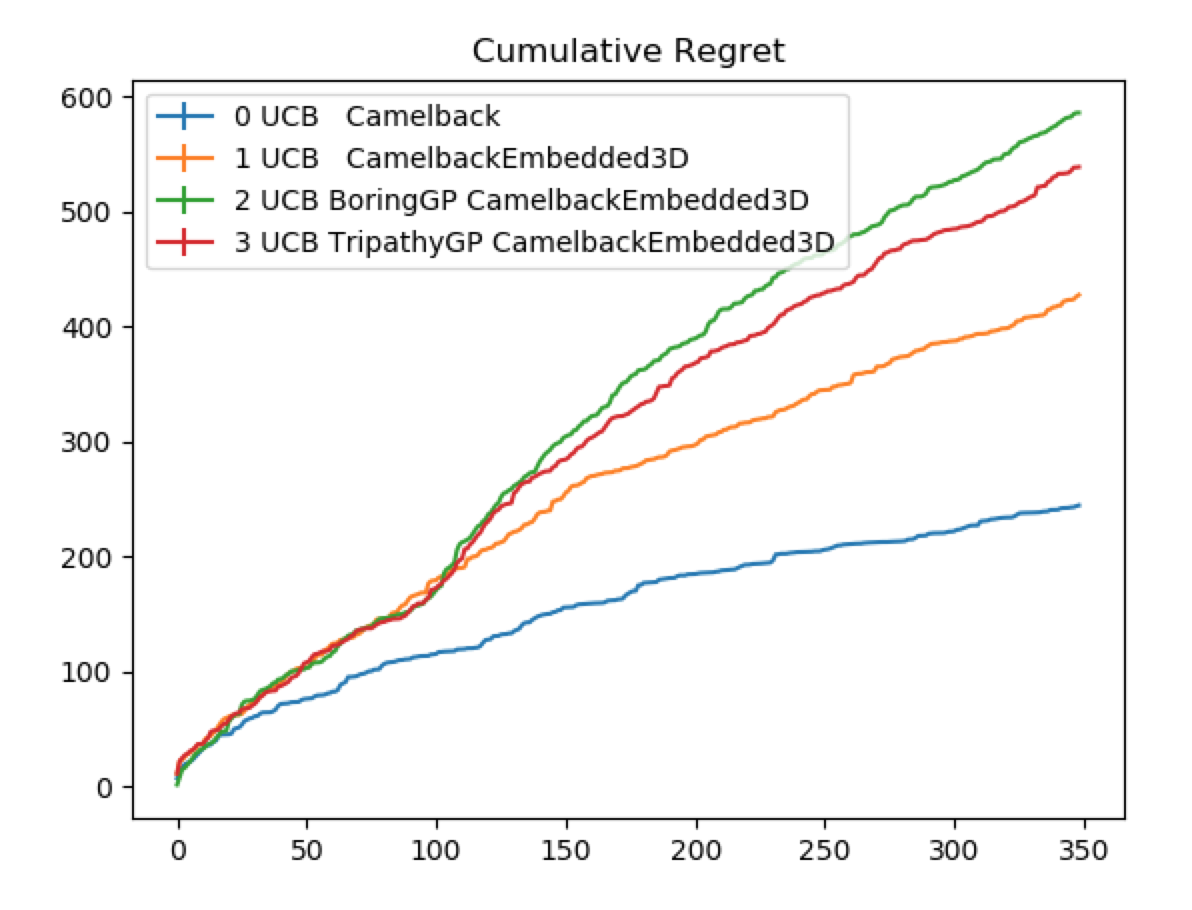
\includegraphics[width=\textwidth]{W_hat_tripathy/Camelback3D_1}
        \label{fig:tiger}
        \caption{Run 2}
    \end{subfigure}   
        \caption{UCB on a 2D Camelback function embedded in 3D space.
          We apply Tripathy's algorithm to find a projection matrix $W$.}
\end{figure}

One can see that the subspace projection of Tripathy's method from 3D to 2D is not efficient. 
The difference between BORING and Tripathy is marginal, as they both rely on a similar algorithm.
This is an indication that the subspace projection is not close to the real subspace, but potentially finds a subspace which is acceptable when higher dimensions are taken into consideration.
To investigate this further, we increase the dimensionality of the domain in the next section.

\subsection{Camelback embedded in 5D}

\def\WCamelback5D{
\begin{bmatrix}
     -0.31894555 & 0.78400512 & 0.38970008 & 0.06119476 & 0.35776912 \\,
     -0.27150973 & 0.066002 & 0.42761931 & -0.32079484 &-0.79759551
\end{bmatrix}}

\begin{equation}
f(z_1, z_2) = \left( 4 - 2.1 * z_1^2 + \frac{z_1^4}{3} \right)  z_1^2 + z_1 *  z_2 + \left(-4 + 4 * z_2^2 \right) * z_2^2
\end{equation} \\

where we have \\
$z = \left( \WCamelback5D^T x \right) $, and $ x \in \mathbf{R}^5$, $W \in \mathbf{R}^{2 \times 5}$
and where $z_1$ denotes the first entry of the $z$ vector, and $z_2$ denotes the second element of the $z$ vector.

\paragraph{Assume $\hat{W} = W_{\text{true}}$}: The following shows how tripathy performs when we assume perfect projection-matrix identification.

\begin{figure}[H]
  \centering
      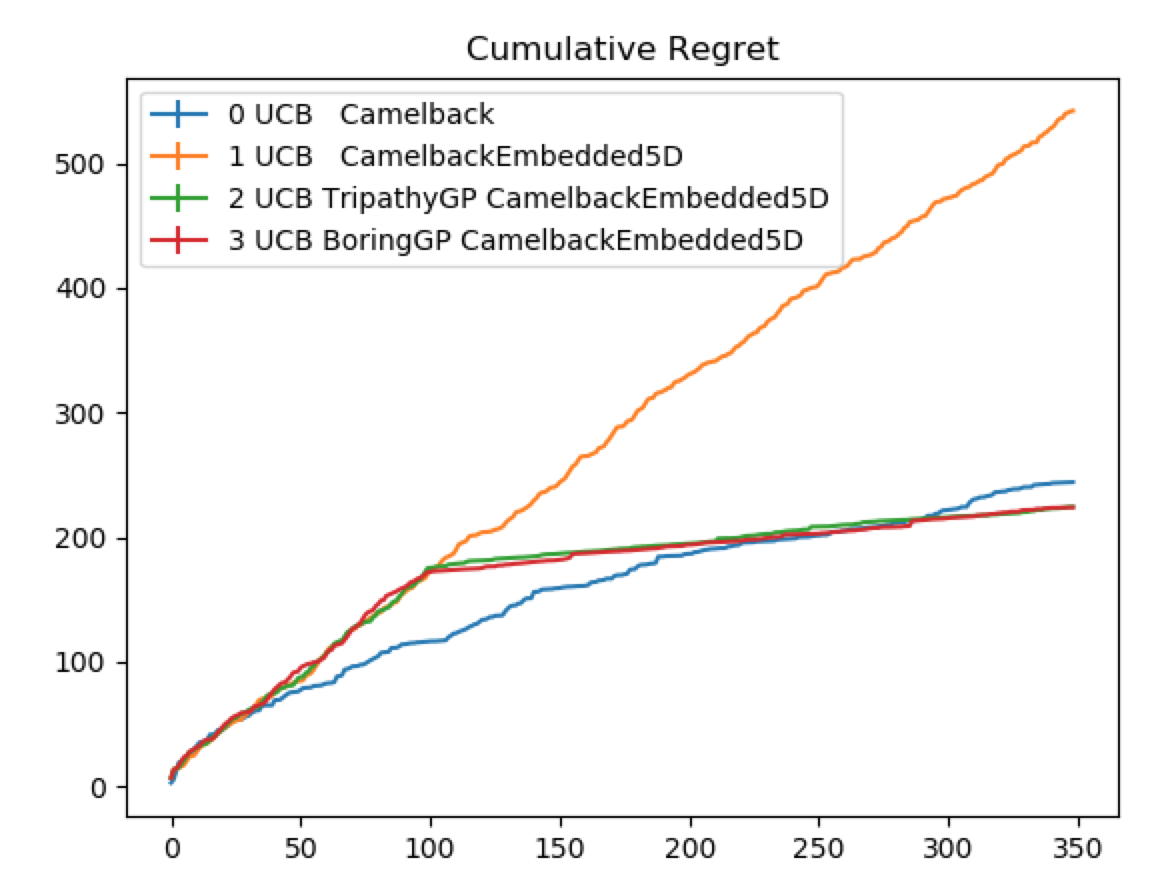
\includegraphics[width=0.5\textwidth]{reference_W_true/Camelback5D}
  \caption{UCB on a 2D Camelback function embedded in 5D space.
  This is when we assume that Tripathy finds the real projection matrix $W_{\text{true}}$}
\end{figure}

The linear curve may be the result of kernel parameters that were not set very well, which may lead to the same point chosen repeatedly over and over again.
However, because the algorithm chooses these kernel parameters, I do not modify these to get square-root behaved UCB curves.

\paragraph{Assume $\hat{W} \neq W_{\text{true}}$}: The following curves present the performance of UCB when subspace identification is part of the optimization process.

\begin{figure}[H]
    \centering
    \begin{subfigure}[b]{0.40\textwidth}
        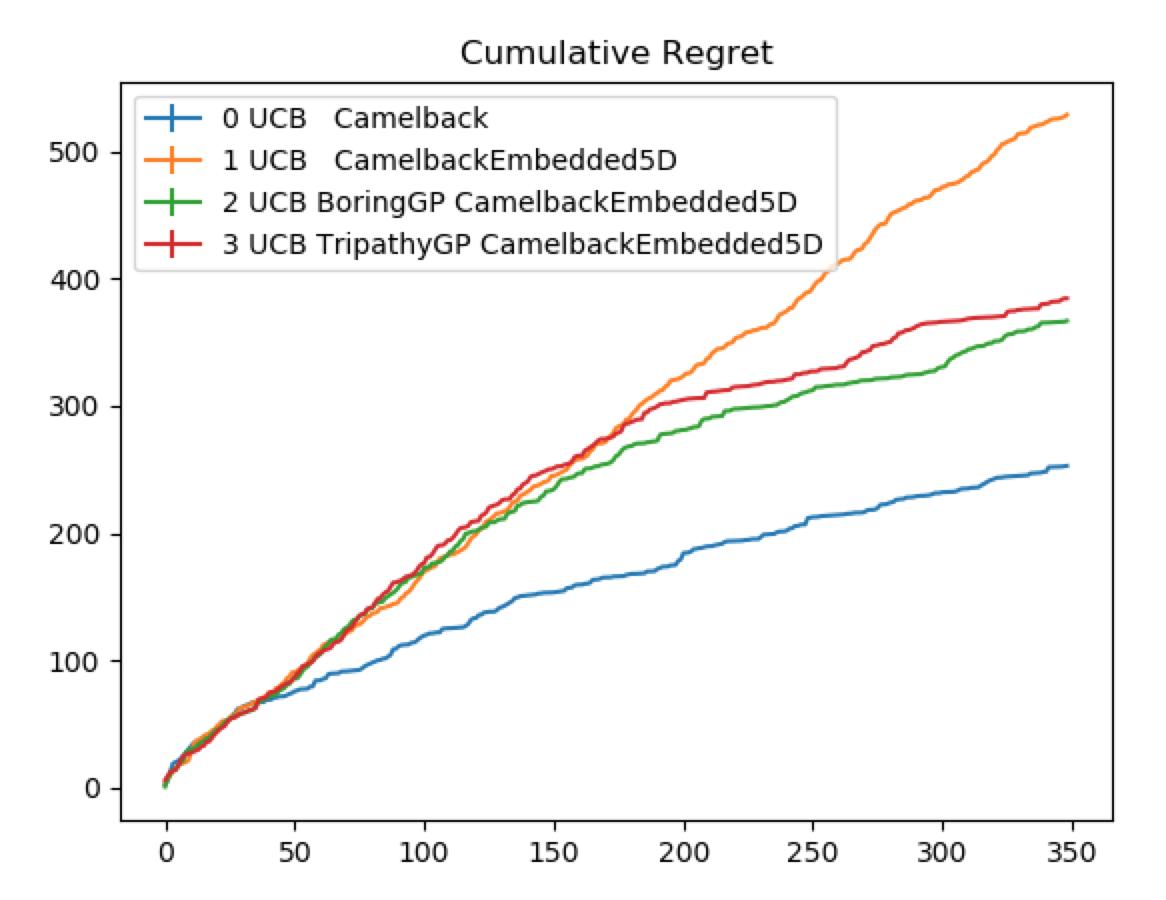
\includegraphics[width=\textwidth]{W_hat_tripathy/Camelback5D_0}
        \label{fig:gull}
        \caption{Run 1}
    \end{subfigure}
    %add desired spacing between images, e. g. ~, \quad, \qquad, \hfill etc. 
      %(or a blank line to force the subfigure onto a new line)
    \begin{subfigure}[b]{0.40\textwidth}
        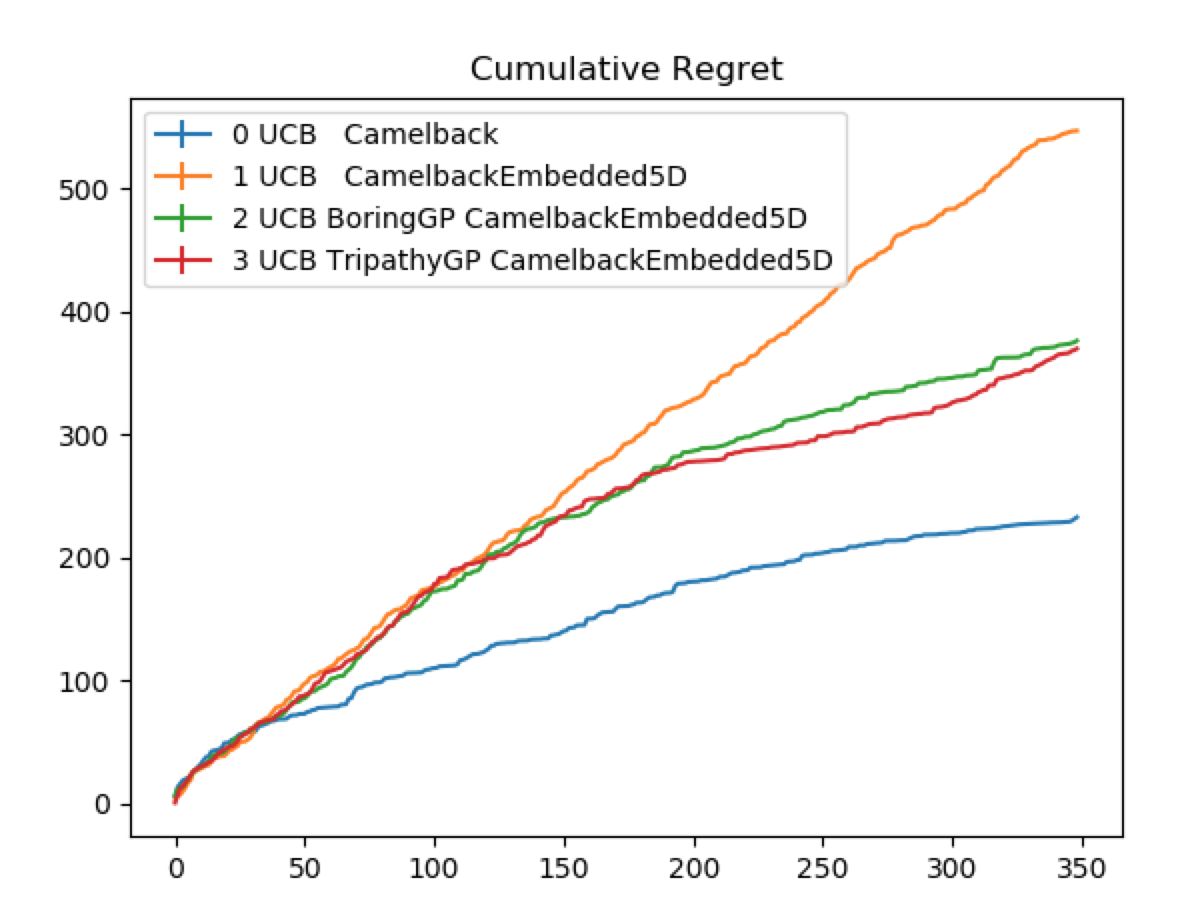
\includegraphics[width=\textwidth]{W_hat_tripathy/Camelback5D_1}
        \label{fig:tiger}
        \caption{Run 2}
    \end{subfigure}   
           \caption{UCB on a 2D Camelback function embedded in 5D space.
  This is when we apply Tripathy's algorithm to find a projection matrix $W$, that is acceptable for optimization, but is not near close to the real projection matrix.}
\end{figure}

One can see for higher dimensions, Tripathy's method performs well, as it can reduce the dimensionality of the optimization problem.
However, one can see that the regret achieved from the empirical projection-matrix identification (the real projection-matrix is not found) is much higher.
This poses the question of how well the found projection matrix is compared to the real projection matrix.
I analyze the log-likelihood of the GP to get a quick answer. \\

\textbf{The log likelihood of the GP w.r.t the collected data points} of the Tripathy GP with the real matrix is not comparable to the log-likelihood of the GP of the Tripathy model, where the active projection matrix is calculated using the algorithm.
For different runs, the log-likelihood of the GP including the real matrix is at $-2$ and $-389$, whereas the log-likelihood of the GP with the estimated projection matrix is at $-0.92$ and $-102$. 
Although the values $-2$ and $-0.92$ are close to each other, the pair ($-389$, $-102$) shows that the subspace identification task for this algorithm is much more unstable than that for the parabola.
In the following subsection, I will investigate this issue further.

\subsection{Log-Likelihood and Angle difference measures}

An interesting quantity to take into consideration is the log-likelihood of the sampled data with respect to the GP, and the angle between the found projection matrix, and the real projection matrix.
In the following, I describe how these quantities change over a function of time.
More specifically, the time refers to the number of steps that I allow for Tripathy's method to optimize over these parameters.

\paragraph{Parabola}

From the graphs, we can see that the parabola always seems to converge at a projection that is at a 45° to the real projection matrix. 
Intuitively, this seems odd.
One should notice, that the maximum of the optimization problem is the same when the space is rotated by 45°.
Another explanation could be that 100 data points on a 2D space are numerous enough, such that any matrix that does not directly map to the nullspace of the real projection matrix is an acceptable matrix.
Why the algorithm always converges at a matrix at 45° to the real projection matrix, would be unclear however in this case.

\begin{figure}[H]
    \centering
    \begin{subfigure}[b]{0.4\textwidth}
        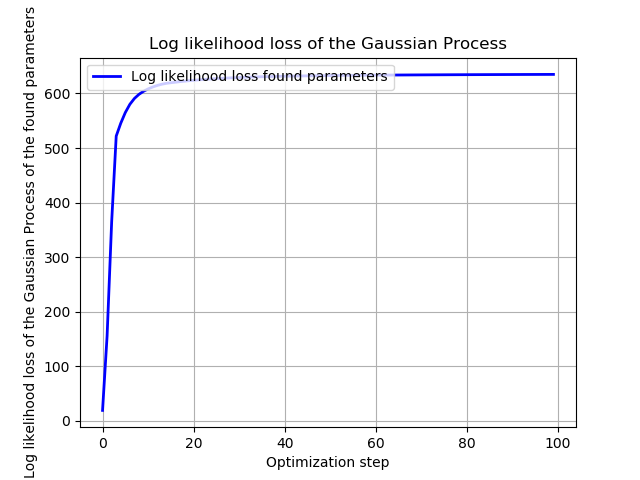
\includegraphics[width=\textwidth]{angles_loss/parabola/Parabola-2D-_1D_20_695_max_run__multiple_loss}
        \label{fig:gull}
           \caption{The momentary $W$ from tripathy's algorithm, and it's log-likelihood w.r.t. the sampled data}
    \end{subfigure}
    \quad
        \begin{subfigure}[b]{0.40\textwidth}
        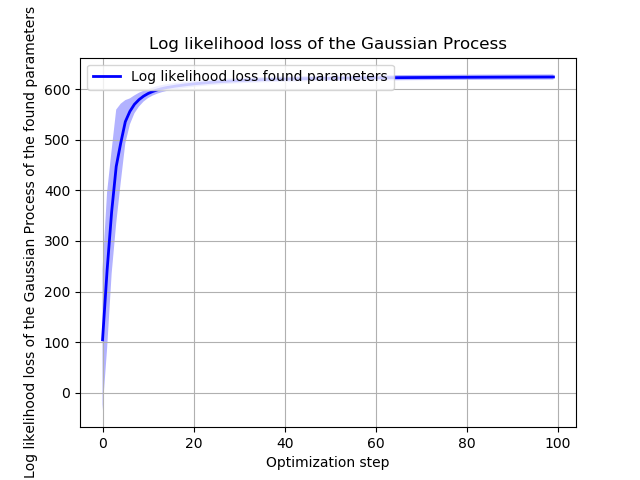
\includegraphics[width=\textwidth]{angles_loss/parabola/Parabola-2D-_1D_20_695_multiple_loss}
        \label{fig:gull}
           \caption{The average of all momentary $W$ from Tripathy's algorithm, and it's log-likelihood to the sampled data}
    \end{subfigure}    \vskip\baselineskip
        \begin{subfigure}[b]{0.40\textwidth}
        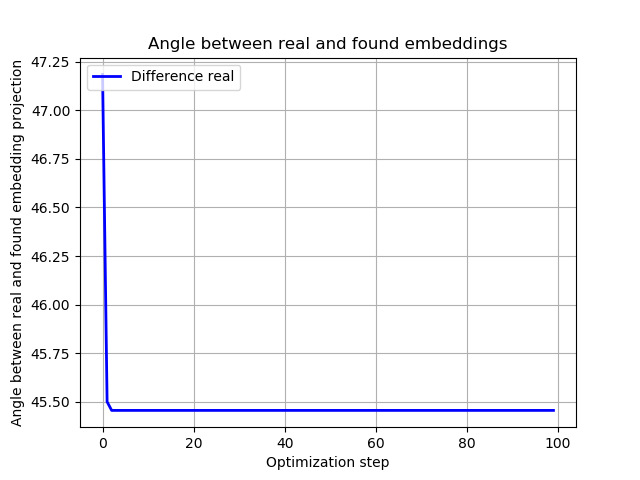
\includegraphics[width=\textwidth]{angles_loss/parabola/Parabola-2D-_1D_20_695_max_run__multiple_angle}
        \label{fig:gull}
           \caption{The momentary $W$ from Tripathy's algorithm, and its angle to the real projection matrix}
    \end{subfigure}
        \quad
        \begin{subfigure}[b]{0.40\textwidth}
        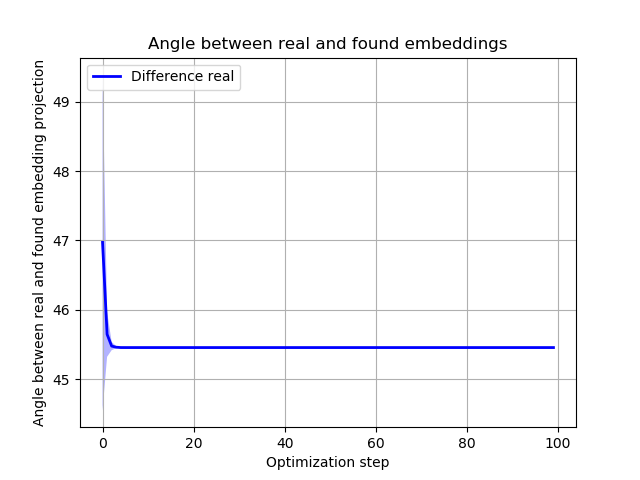
\includegraphics[width=\textwidth]{angles_loss/parabola/Parabola-2D-_1D_20_695_multiple_angle}
        \label{fig:gull}
           \caption{The average of all momentary $W$ from Tripathy's algorithm, and it's angle to the real projection matrix}
          \end{subfigure}
    \caption{Log-Likelihood (top) and Angle (bottom) performance measures for a 1D Parabola embedded in a 2D space.
    The left graphs show the values for the run that was chosen as the "found" projection matrix.
    The right graphs show the average values over all restarts of tripathy's method.
    }\label{fig:animals}
\end{figure}

\paragraph{Camelback}
Because from the UCB experiments, we assume Camelback to be more unstable, we show the results of two independent runs that exhibit different behavior.
This is evidence, which Tripathy's algorithm on Camelback does not run stable, and has high variance (i.e., is not as robust).


\begin{figure}[H]
    \centering
    \begin{subfigure}[b]{0.40\textwidth}
        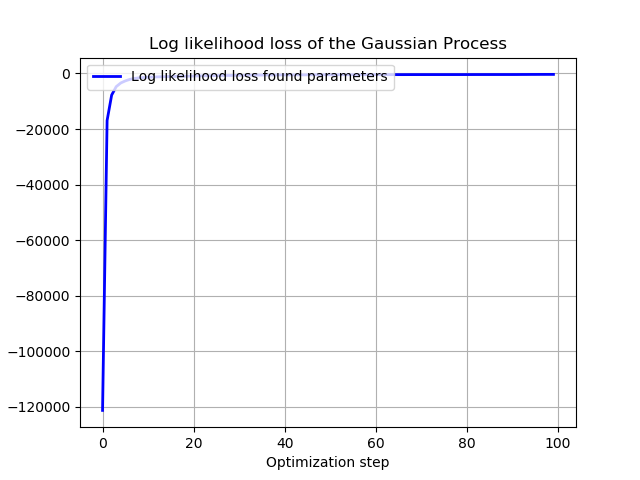
\includegraphics[width=\textwidth]{angles_loss/camelback/run1/Camelback-5D-_2D_20_175_max_run__multiple_loss}
        \label{fig:gull}
                           \caption{The momentary $W$ from tripathy's algorithm, and it's log-likelihood w.r.t the sampled data}
    \end{subfigure}
       \quad
   \begin{subfigure}[b]{0.40\textwidth}
        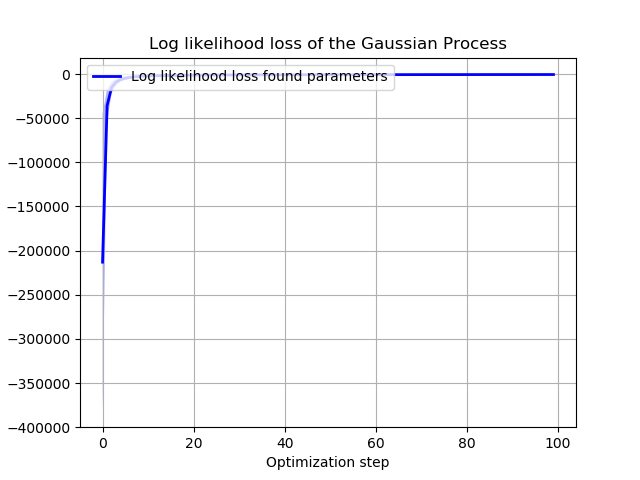
\includegraphics[width=\textwidth]{angles_loss/camelback/run1/Camelback-5D-_2D_20_175_multiple_loss}
        \label{fig:gull}
                           \caption{The average of all momentary $W$ from tripathy's algorithm, and it's log-likelihood w.r.t the sampled data}
    \end{subfigure} 
 \vskip\baselineskip
        \centering
    \begin{subfigure}[b]{0.40\textwidth}
        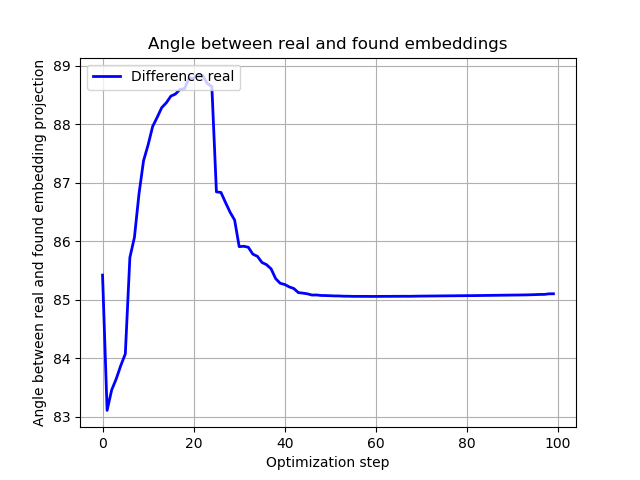
\includegraphics[width=\textwidth]{angles_loss/camelback/run1/Camelback-5D-_2D_20_175_max_run__multiple_angle}
        \label{fig:gull}
               \caption{The momentary $W$ from Tripathy's algorithm, and its angle to the real projection matrix}
    \end{subfigure}
        \quad
        \begin{subfigure}[b]{0.40\textwidth}
        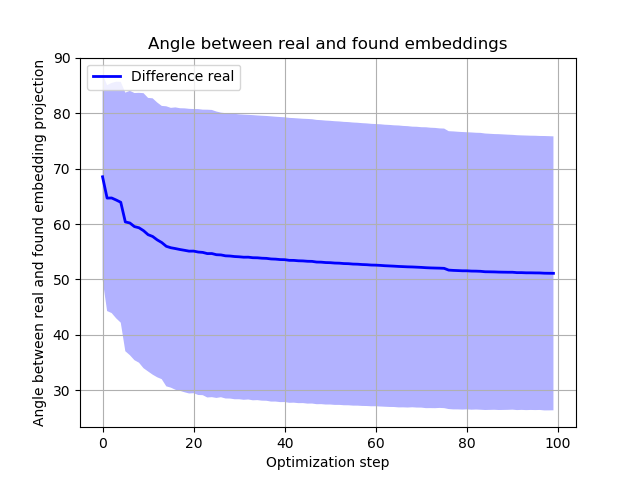
\includegraphics[width=\textwidth]{angles_loss/camelback/run1/Camelback-5D-_2D_20_175_multiple_angle}
        \label{fig:gull}
                           \caption{The average of all momentary $W$ from Tripathy's algorithm, and it's angle to the real projection matrix}
    \end{subfigure}
    \caption{Log-Likelihood (top) and Angle (bottom) performance measures for a 2D Camelback embedded in a 5D space.
    The left graphs show the values for the run that was chosen as the "found" projection matrix.
    The right graphs show the average values over all restarts of Tripathy's method.
    These are the results for run 1.
    }\label{fig:animals}
\end{figure}

\begin{figure}[H]
\center
    \begin{subfigure}[b]{0.40\textwidth}
        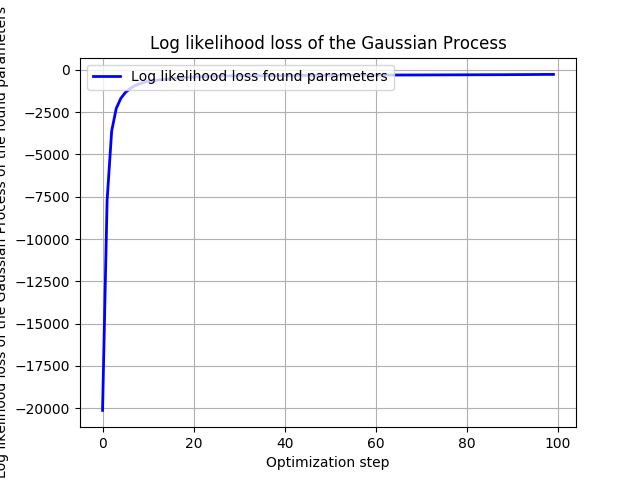
\includegraphics[width=\textwidth]{angles_loss/camelback/run2/Camelback-5D-_2D_20_489_max_run__multiple_loss}
        \label{fig:tiger}                          
         \caption{The momentary $W$ from tripathy's algorithm, and it's log-likelihood w.r.t the sampled data}
    \end{subfigure}   
        \quad
    \begin{subfigure}[b]{0.40\textwidth}
        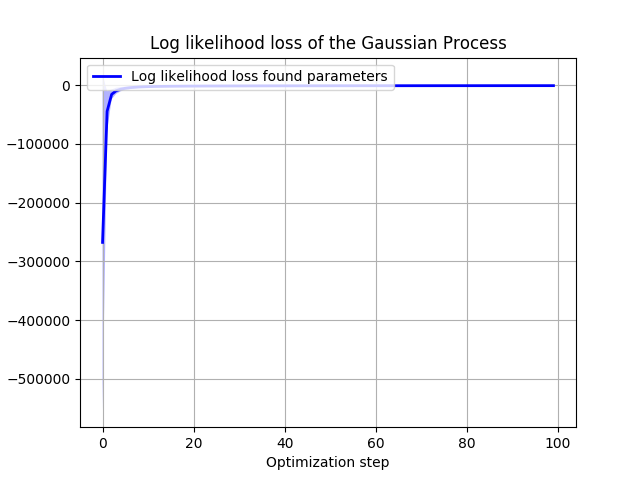
\includegraphics[width=\textwidth]{angles_loss/camelback/run2/Camelback-5D-_2D_20_489_multiple_loss}
        \label{fig:tiger}
               \caption{The momentary $W$ from tripathy's algorithm, and it's angle to the real projection matrix}
    \end{subfigure}   
 \vskip\baselineskip
         \centering
             \begin{subfigure}[b]{0.40\textwidth}
        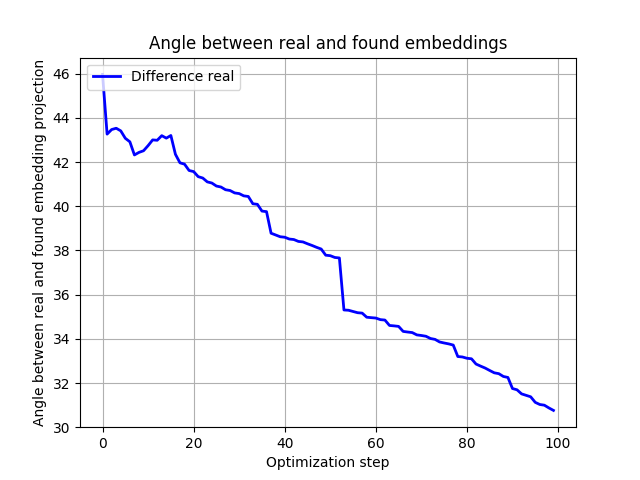
\includegraphics[width=\textwidth]{angles_loss/camelback/run2/Camelback-5D-_2D_20_489_max_run__multiple_angle}
        \label{fig:tiger}                           
        \caption{The average of all momentary $W$ from tripathy's algorithm, and it's log-likelihood w.r.t the sampled data}
    \end{subfigure}
        \quad
    \begin{subfigure}[b]{0.40\textwidth}
        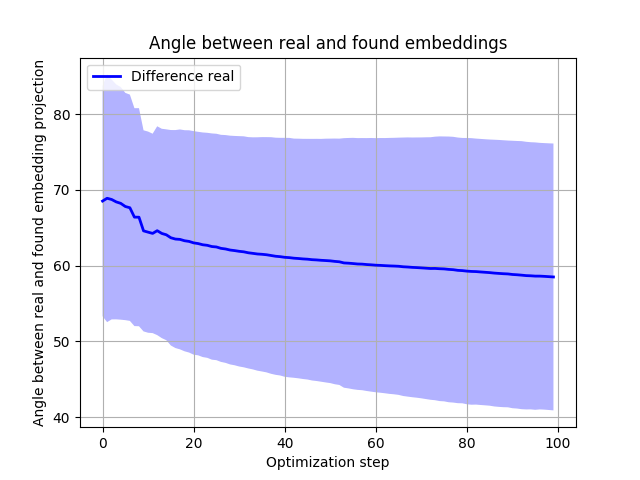
\includegraphics[width=\textwidth]{angles_loss/camelback/run2/Camelback-5D-_2D_20_489_multiple_angle}
        \label{fig:tiger}
               \caption{The average of all momentary $W$ from Tripathy's algorithm, and it's angle to the real projection matrix}
    \end{subfigure}   
        \caption{Log-Likelihood (top) and Angle (bottom) performance measures for a 2D Camelback embedded in a 5D space.
    The left graphs show the values for the run that was chosen as the "found" projection matrix.
    The right graphs show the average values over all restarts of Tripathy's method.
    These are the results for run 2.
    }\label{fig:animals}
\end{figure}


\paragraph{Sinusoidal}: 
Although we do not show the UCB curves for the sinusoidal (which also prove to be successful, when this 2d function is hidden within a 5D space), good results can be obtained for subspace identification.

\begin{figure}[H]
\center
    \begin{subfigure}[b]{0.40\textwidth}
        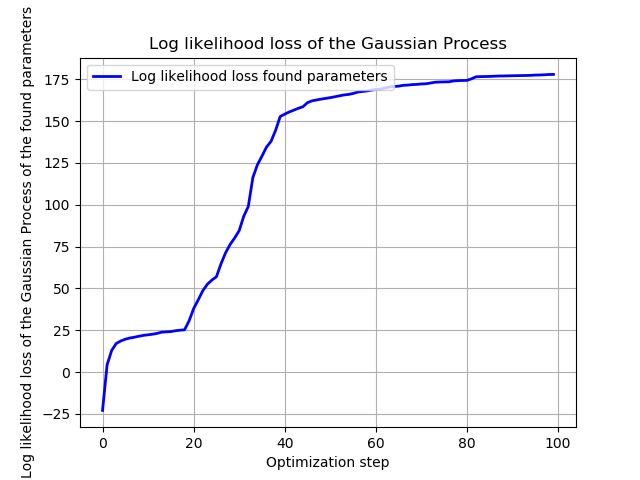
\includegraphics[width=\textwidth]{angles_loss/sinusoidal/Sinusoidal-5D-_2D_20_341_max_run__multiple_loss}
        \label{fig:gull}
         \caption{The momentary $W$ from tripathy's algorithm, and it's log-likelihood w.r.t the sampled data}
    \end{subfigure}
       \quad
        \begin{subfigure}[b]{0.40\textwidth}
        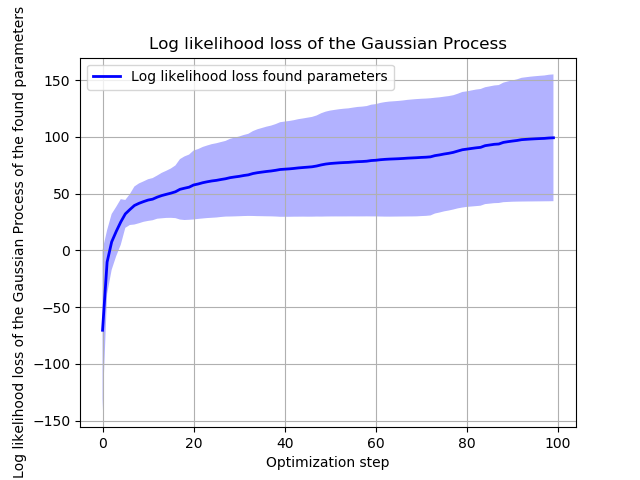
\includegraphics[width=\textwidth]{angles_loss/sinusoidal/Sinusoidal-5D-_2D_20_341_multiple_loss}
        \label{fig:gull}
        \caption{The average of all momentary $W$ from tripathy's algorithm, and it's log-likelihood w.r.t the sampled data}
    \end{subfigure}

 \vskip\baselineskip
         \centering           

    \begin{subfigure}[b]{0.40\textwidth}
        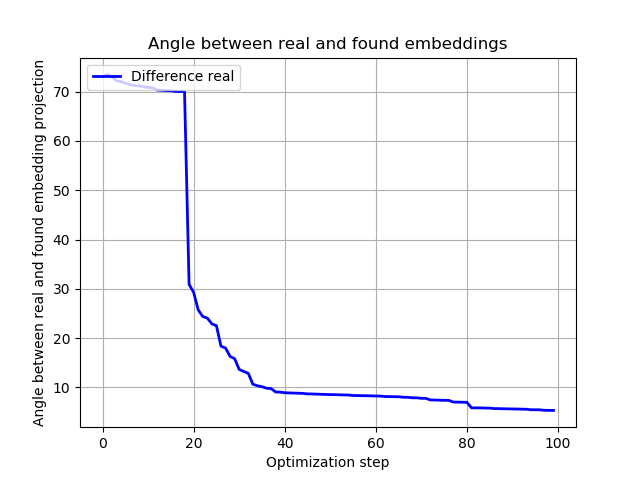
\includegraphics[width=\textwidth]{angles_loss/sinusoidal/Sinusoidal-5D-_2D_20_341_max_run__multiple_angle}
        \label{fig:gull}
               \caption{The momentary $W$ from Tripathy's algorithm, and its angle to the real projection matrix}
    \end{subfigure}
        \quad
    \begin{subfigure}[b]{0.40\textwidth}
        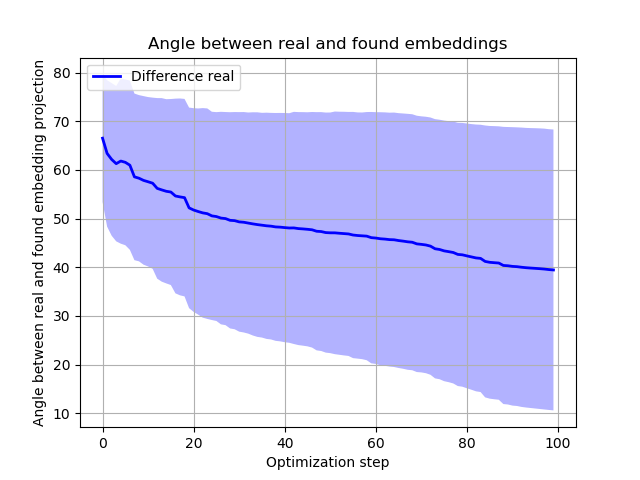
\includegraphics[width=\textwidth]{angles_loss/sinusoidal/Sinusoidal-5D-_2D_20_341_multiple_angle}
        \label{fig:gull}
               \caption{The average of all momentary $W$ from Tripathy's algorithm, and it's angle to the real projection matrix}
    \end{subfigure}
           
        \caption{Log-Likelihood (top) and Angle (bottom) performance measures for a 2D Sinusoidal function embedded in a 5D space.
    The left graphs show the values for the run that was chosen as the "found" projection matrix.
    The right graphs show the average values over all restarts of Tripathy's method.
    These are the results for run 2.
    }\label{fig:animals}
\end{figure}

\section{REMBO}

The final algorithm I am investigating is REMBO, as described in chapter 2.
REMBO generally finds proper embeddings under the assumption, that optimization domain is normalized, and scaled to $[-\sqrt{d}, \sqrt{d}]^d$ where $d$ is at least the effective dimensionality of the optimization function at hand. 
The reader should acknowledge that the algorithm that was used to create the below plots only allowed to sample orthogonal matrices (instead of random matrices in REMBO).
This is a detail I noticed too late and could not change timely.
However, running two experiments for each environment with the randomly sampled matrix (without the orthogonality constraint) yielded similar results with a higher number of bad projections.
Because the results were similar besides the higher number of bad projections, I decided to keep the plots including the orthogonally sampled matrix. \\

I shortly present results for UCB that use REMBO as their optimization algorithm.
The high probability of failing implies a high variance amongst runs. 
As such, I perform three runs for each function addressed in the above section.

\paragraph{Parabola}
As one can see, REMBO usually finds an embedding that is acceptable and accelerates the optimization process.
However, run two shows that it can also fail in the simplest case of the parabola.
In this regards, Tripathy's method is more robust, as it does use some heuristic to check if the chosen matrix delivers good results.


\begin{figure}[H]
\center
    \begin{subfigure}[b]{0.30\textwidth}
        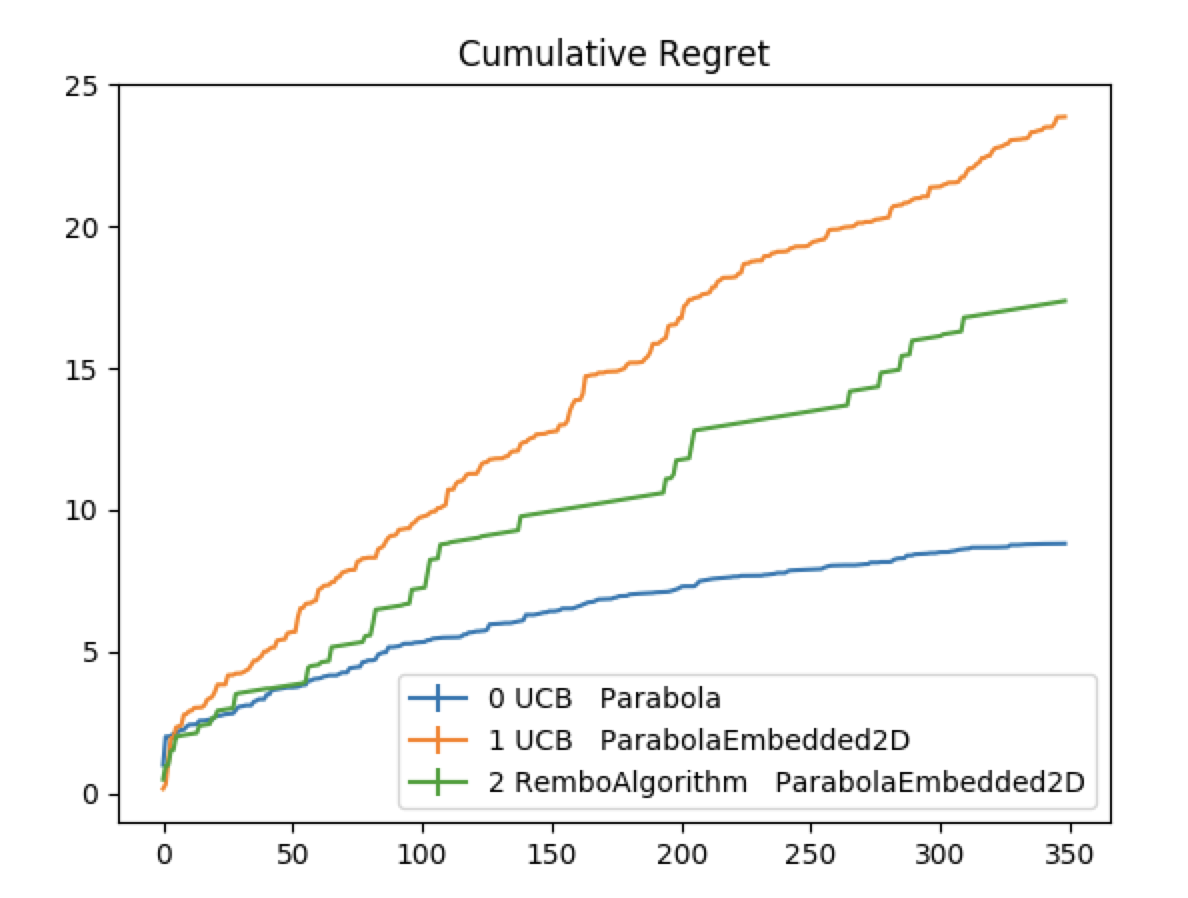
\includegraphics[width=\textwidth]{rembo/Parabola_run0}
        \label{fig:gull}
         \caption{Run 1}
    \end{subfigure}
        \begin{subfigure}[b]{0.30\textwidth}
        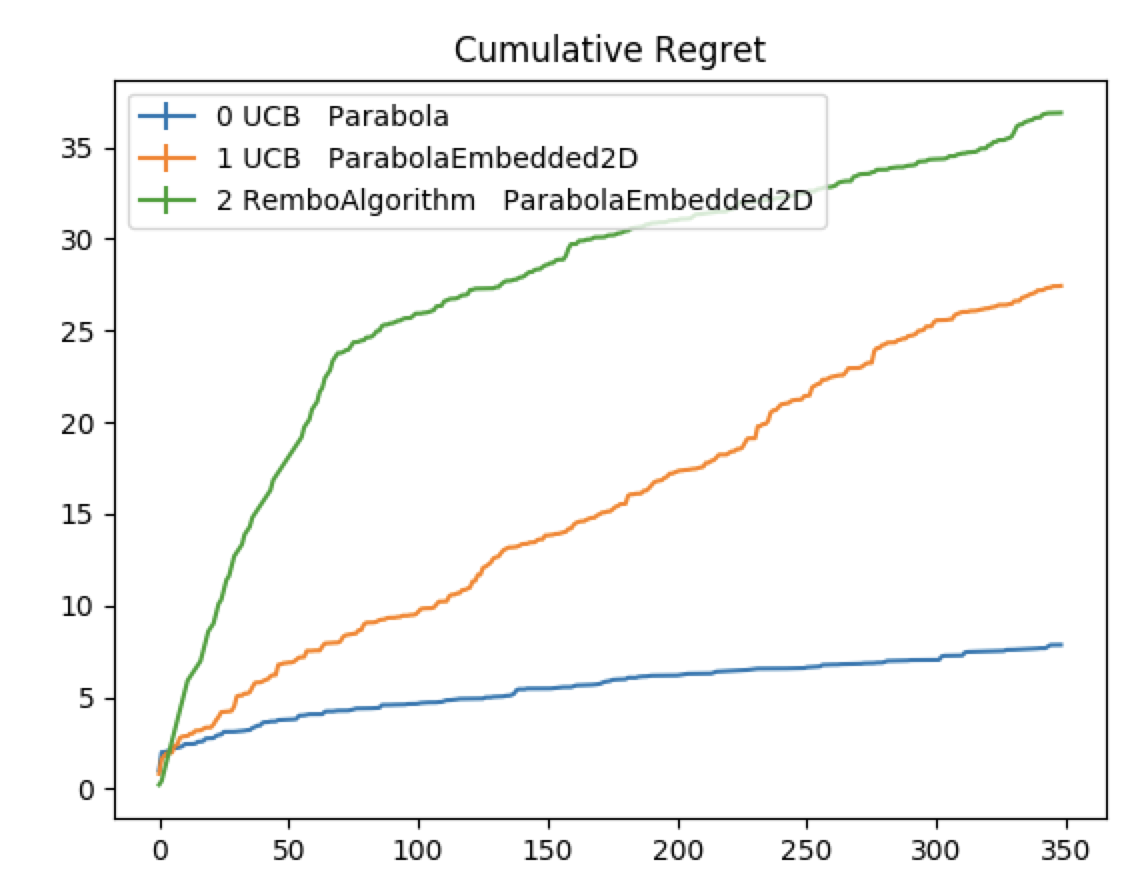
\includegraphics[width=\textwidth]{rembo/Parabola_run1}
        \label{fig:gull}
        \caption{Run 2}
    \end{subfigure}
    \begin{subfigure}[b]{0.30\textwidth}
        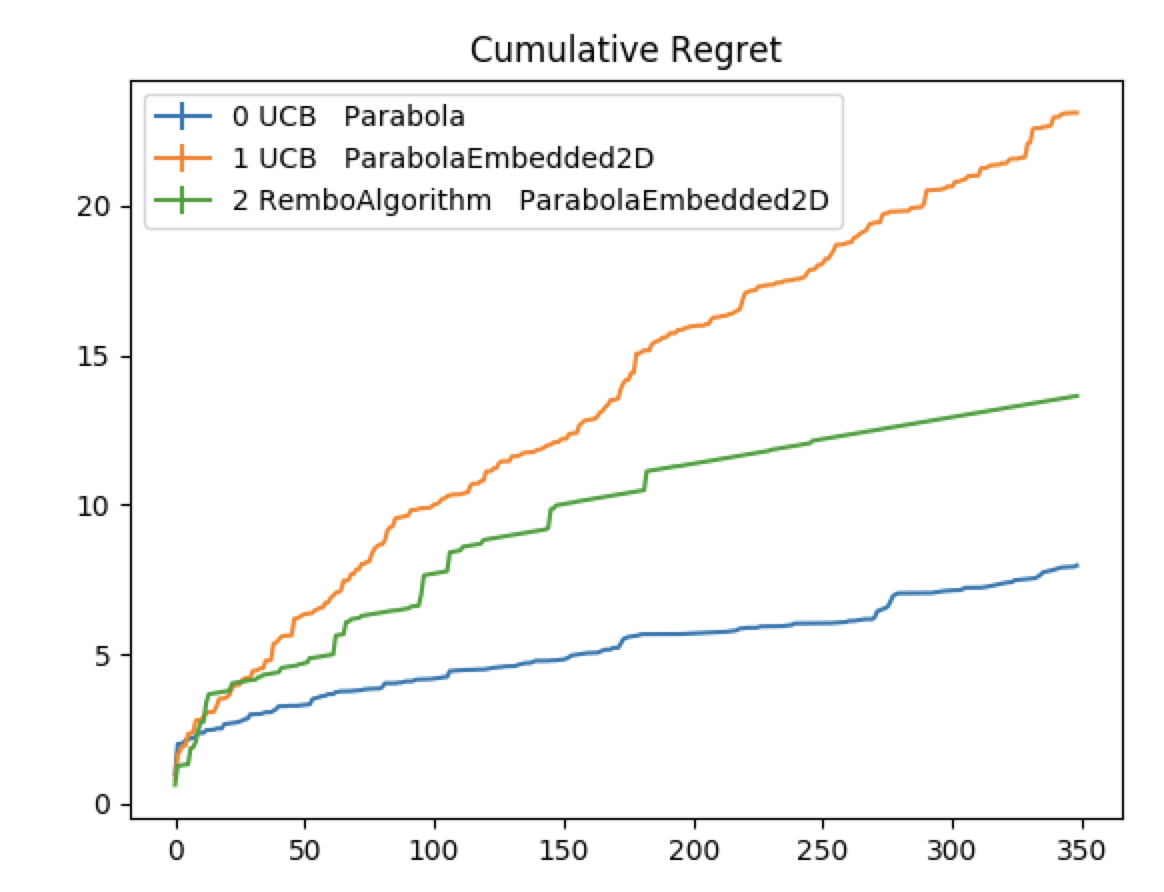
\includegraphics[width=\textwidth]{rembo/Parabola_run2}
        \label{fig:gull}
               \caption{Run 3}
    \end{subfigure}
        \caption{UCB using REMBO on a 1D Parabola embedded in a 2D space.
    }\label{fig:animals}
\end{figure}

\paragraph{Camelback3D}
This example illustrates how REMBO can find an acceptable subspace.
However, the straight lines are an indication for the hyperparameters to be no well chosen.
I do not allow hyperparameter optimization, for the reason such that the results may be comparable to the other algorithm's results.
As one can see, Camelback3D also provides a difficult for REMBO, although REMBO does find an acceptable subspace projection.

\begin{figure}[H]
\center
    \begin{subfigure}[b]{0.30\textwidth}
        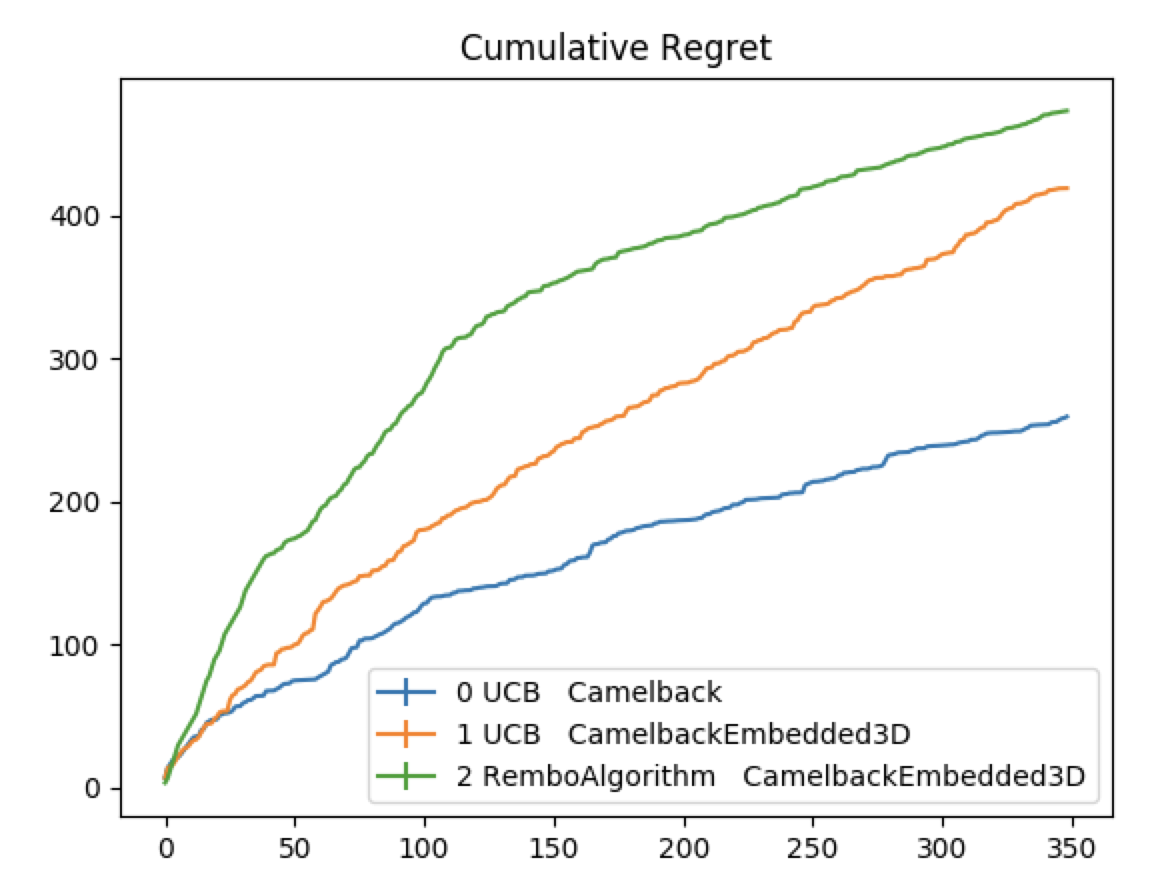
\includegraphics[width=\textwidth]{rembo/Camelback3D_run0}
        \label{fig:gull}
         \caption{Run 1}
    \end{subfigure}
        \begin{subfigure}[b]{0.30\textwidth}
        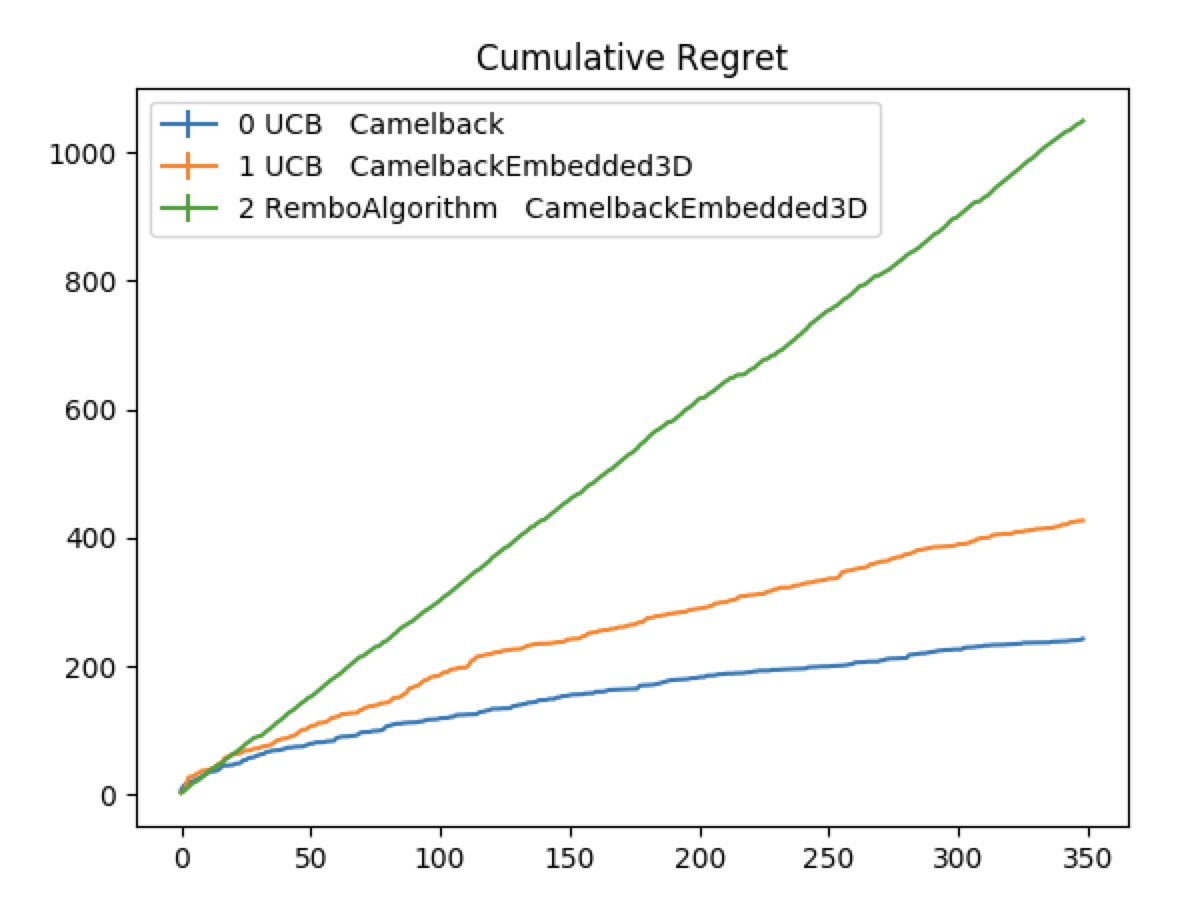
\includegraphics[width=\textwidth]{rembo/Camelback3D_run1}
        \label{fig:gull}
        \caption{Run 2}
    \end{subfigure}
    \begin{subfigure}[b]{0.30\textwidth}
        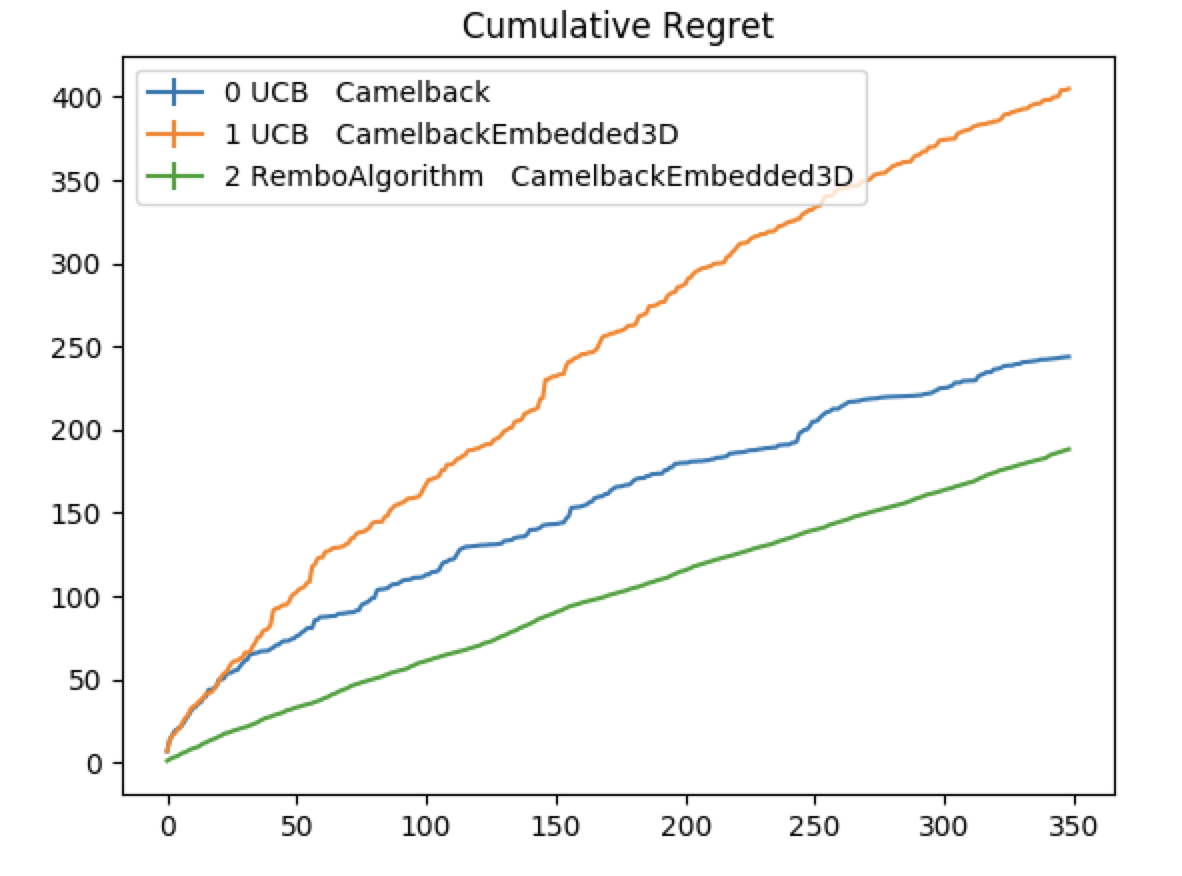
\includegraphics[width=\textwidth]{rembo/Camelback3D_run2}
        \label{fig:gull}
               \caption{Run 3}
    \end{subfigure}
        \caption{UCB using REMBO on a 2D Camelback embedded in a 3D space.
    }\label{fig:animals}
\end{figure}

\paragraph{Camelback5D}
The linearity of the UCB curves is still attained.
Similar to the result with Tripathy's method, REMBO can reduce the dimensionality of the subspace in almost any case.
The effectiveness of this reduction can be small though.
The viewer can recognize well that there is a high variance in the performance amongst runs.
This emphasizes how important the interleaved runs are, even though the number of data samples per projection is divided by the total number of projection (i.e., there is slower learning of the GP surface. However, dimensionality reduction is successful).

\begin{figure}[H]
\center
    \begin{subfigure}[b]{0.30\textwidth}
        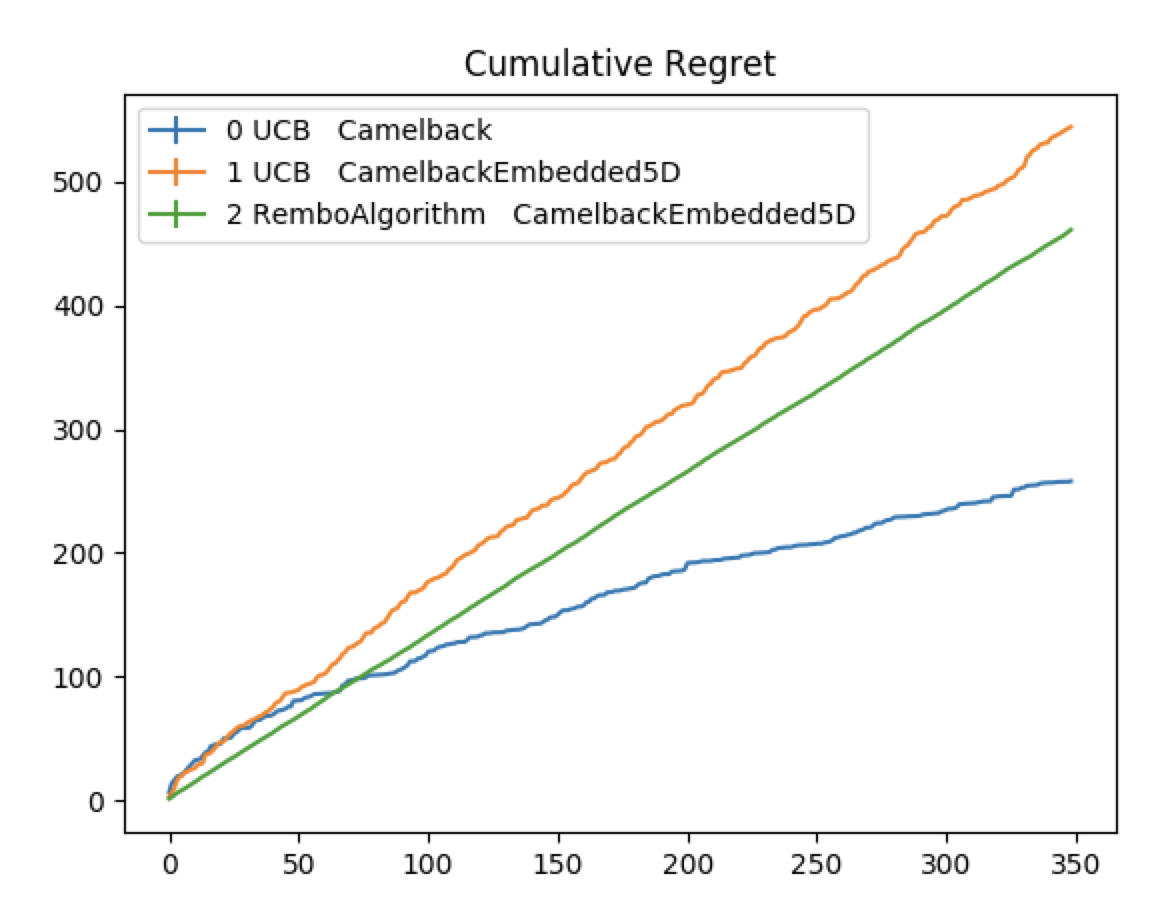
\includegraphics[width=\textwidth]{rembo/Camelback5D_run0}
        \label{fig:gull}
         \caption{Run 1}
    \end{subfigure}
        \begin{subfigure}[b]{0.30\textwidth}
        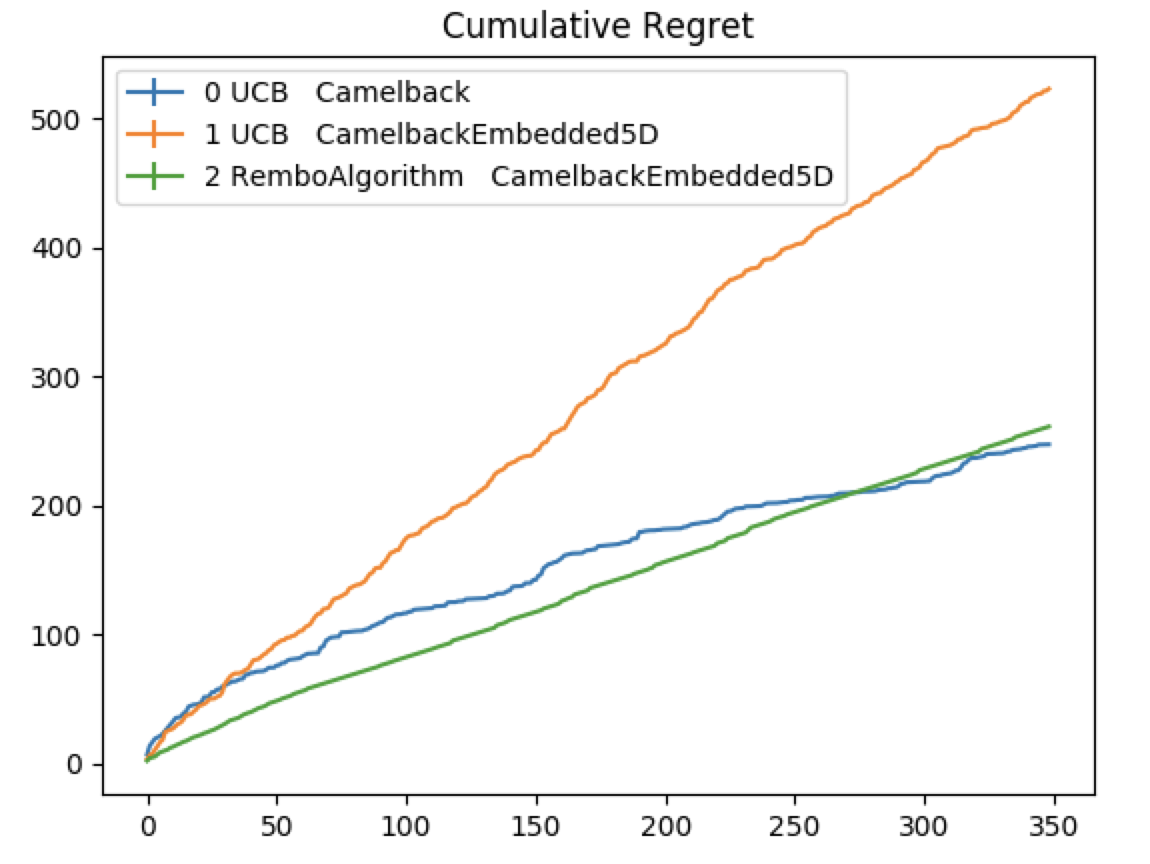
\includegraphics[width=\textwidth]{rembo/Camelback5D_run1}
        \label{fig:gull}
        \caption{Run 2}
    \end{subfigure}
    \begin{subfigure}[b]{0.30\textwidth}
        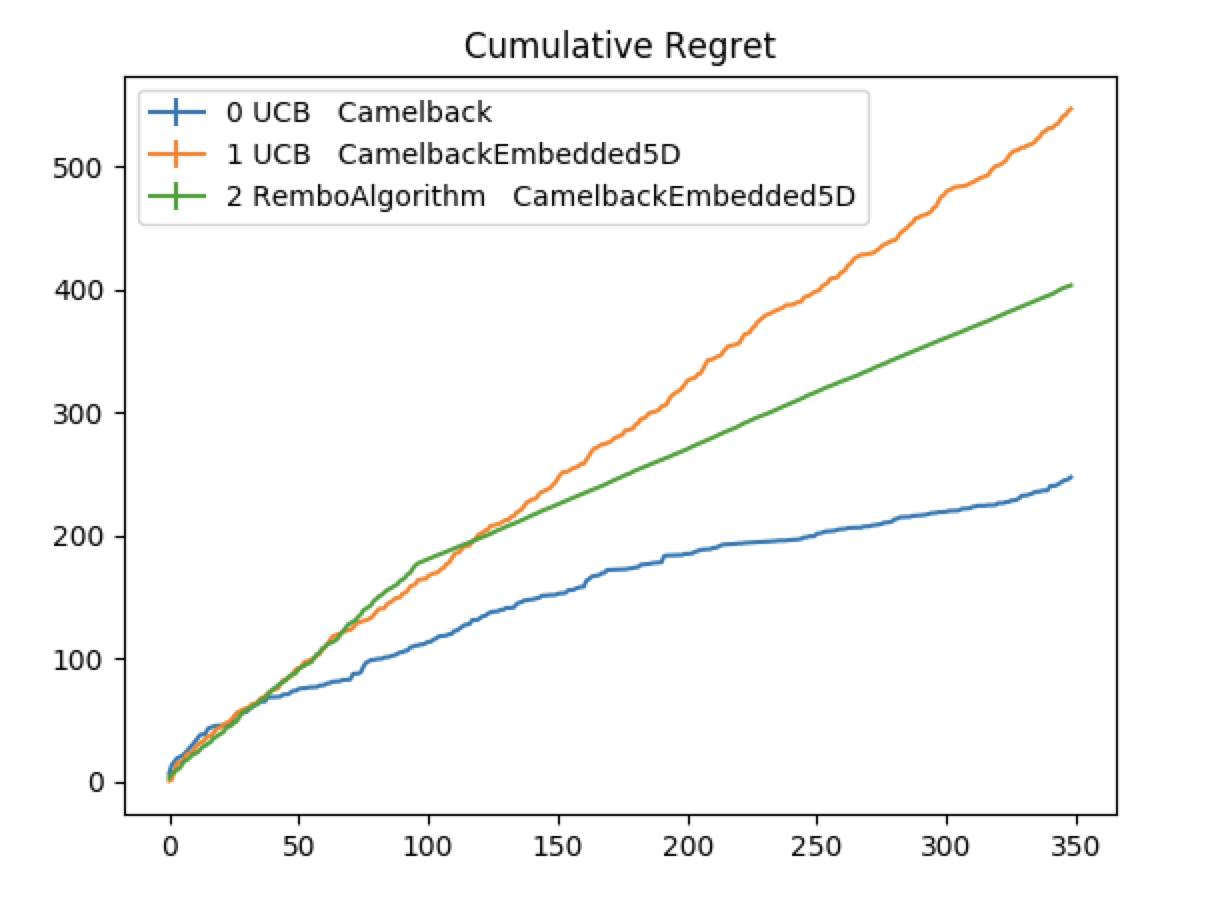
\includegraphics[width=\textwidth]{rembo/Camelback5D_run2}
        \label{fig:gull}
               \caption{Run 3}
    \end{subfigure}
        \caption{UCB using REMBO on a 2D Camelback embedded in a 5D space.
    }\label{fig:animals}
\end{figure}


\section{Qualitative evaluation}
It is interesting to see, that amongst the 1000 restarts that I generated some of the resulting matrices are close to the real projection matrix up to an absolute value of 0.01.
However, because the algorithm decides to choose the matrix with the highest likelihood, Tripathy's algorithm, in general, does not select these matrices but chooses a matrix that is not amongst the matrices that are very similar to the real matrices.

\subsection{Feature selection}
The goal of this task is to see if the revised active subspace identification algorithms can effectively apply feature selection.
For this task, I set up a function $ f $ that looks as follows:

\def\B{
\begin{bmatrix}
    (x - a_0)^2 \\
    (y - a_1)^2
\end{bmatrix}}

\begin{equation} \label{eq:FeatureExtension}
f \left( W \B \right) \approx g \left( x \right)
\end{equation} 

where $x_0, x_1$ are constants. \\

For this specific experiment, the function $f$ is chosen to be a one-dimensional parabola. 
As such, $W$ is chosen as a matrix on the Stiefel manifold with dimensions $\mathbf{R}^{d \times D}$.

Doing a feature extension over $x$ and $y$, we can get the following feature representation:

\def\PHI{
\begin{bmatrix}
    x_0^2 \\
    x_1^2 \\
    x_0 \\
    x_1 \\
    1
\end{bmatrix}}


\def\WtoPhi{
\begin{bmatrix}
    w_0 \\
    w_1 \\
    -2 w_0 a_0 \\
    -2 w_1 a_1 \\
    w_0 a_0^2 + w_1 a_1^2
\end{bmatrix}}

\begin{figure}[h]

\begin {minipage}{0.47\textwidth}
  \centering
  \begin{equation}
    \PHI
  \end{equation}
  \caption{Polynomial Kernel applied to vector $[x_0, x_1]$}
\end{minipage}
\hfill
\begin {minipage}{0.47\textwidth}
  \centering
  \begin{equation}
    \WtoPhi
  \end{equation}
  \caption{Corresponding weight matrix equivalent to \ref{eq:FeatureExtension} when applied on a parabola}
\end{minipage}

\end{figure}

To run experiments, I instantiate the "real" matrix, which should be found by the algorithm with the values $w_0 = 0.589$, $w_1 = 0.808$ (randomly sampled as a matrix on the Stiefel manifold), $a_0 = -0.1$, $a_1 = 0.1$ (chosen by me as coefficients). \\

I apply the algorithm 1. from \citep{Tripathy} to identify the active projection matrix.
The optimization algorithm has 50 samples to discover the hidden matrix, which it seemingly does up do a certain degree of accuracy.
Similar results are achieved for repeated tries.
The following figure shows the real matrix, and the matrix the algorithm has found.

\def\realW{
\begin{bmatrix}
    0.589 \\
    0.808 \\
    0.118 \\
    -0.162 \\
    0.823
\end{bmatrix}}

\def\okW1{
\begin{bmatrix}
    -0.355 \\
        -0.533 \\
        -0.908 \\
        0.099 \\
    -0.756 
\end{bmatrix}}

\begin{figure}[h] 
\begin {minipage}{0.47\textwidth}
  \centering
  \begin{equation} \label{fig:realMatrix}
    \realW
  \end{equation}
  \caption{Real matrix}
\end{minipage}
\hfill
\begin {minipage}{0.47\textwidth}
  \centering
  \begin{equation} \label{fig:foundMatrix}
    \okW1
  \end{equation}
  \caption{Matrix found by optimization algorithm}
\end{minipage}
\end{figure}

Although one can see that the element-wise difference between the two matrices \ref{fig:realMatrix} and \ref{fig:foundMatrix} is high (between $0.05$ and $0.15$, one entry is above $1$), one can see that the matrix recovery is successful in finding an approximate structure that resembles the original structure of the features.
One should observe that the found matrix is an approximate solution to the real matrix in the projection. I.e., the matrix found is close to the real matrix, but multiplied by $-1$. \\

Because in this case, I applied the feature selection algorithm on a vector-matrix (only one column), one can quantify the reconstruction of the real matrix through the found matrix by the normalized scalar product.
This quantity is a metric between $0$ and $1$, where $0$ means that both vectors are orthogonal, and $1$ means that both vectors overlap.

\begin{equation}
\text{overlap}(u, v) = \frac{| \langle u, v \rangle |}{\langle u, u \rangle}
\end{equation}
where $u$ is the real vector, and $v$ is the found vector.

Inserting the actual values into the field, we get $0.79$, which is a good value for the feature vector found, and the trained number of data points which is 50. \\
 
 This experiment shows that algorithm 1. from \citep{Tripathy} successfully allows a viable option to other feature selection algorithms, by providing a measure, where the optimal linear projection is found. 
 However, one must notice that other feature selection algorithms (such as SVM \citep{SVMFeature}), are more efficient, and will provide better results with a higher probability if applied on a similar kernel. \\
 
 One observation I made was the increase in the log-likelihood of the data w.r.t. The projection matrix did not correlate with the decrease in the angle between the real vs. the found projection matrix.
 Also, most often, the angle was at around 40 degrees, which means that only slight improvements over an entirely random embedding were made.


\subsection{Subspace identification}
One of the main reasons to use our method is because we allow for subspace identification.
We have the following functions:

\begin{enumerate}
\item 1D Parabola embedded in a 2D space
\item 2D Camelback embedded in a 5D space
\item 2D Sinusoidal and Exponential function embedded in a 5D space
\end{enumerate}

To be able to visualize the points, I proceed with the following procedure:

I generate testing points (points to be visualized) within the 2D-space in a uniform grid.
I then project these testing points to the dimension of the original function ($2d$ for parabola, else $5d$).
I then let each algorithm learn and predict the projection matrix, and GP mean predictions.
If because the transformation from $2D$ space to $5D$ space and GP mean prediction is each bijective, we can visualize the $2D$ points with the GP mean prediction right away.
As such, the dimension of the embedding learned does not have an impact on the visualization.

In the following figures, blue point shows the sampled real function value.
Orange points show the sampled mean prediction of the trained GP.
The GPs were each trained on 100 data points. 
The points shown below were not used for training at any point, as these are included in the test set.

% PARABOLA FUNCTION
\begin{figure}[H]
    \centering
    \begin{subfigure}[b]{0.30\textwidth}
        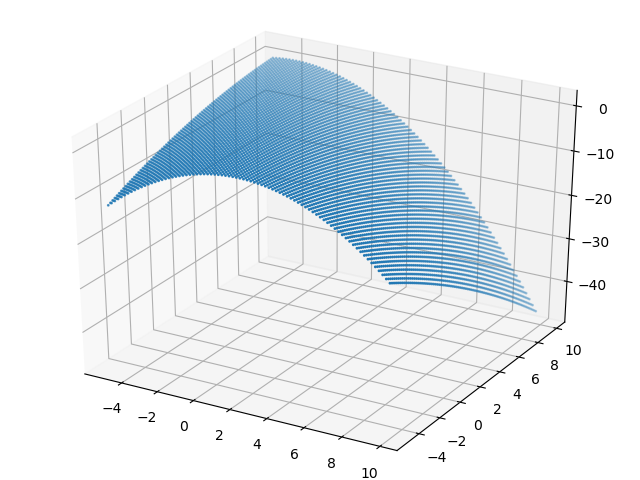
\includegraphics[width=\textwidth]{orig/Parabola-2D-_1D.png}
        \caption{Parabola Original}
        \label{fig:gull}
    \end{subfigure}
    %add desired spacing between images, e. g. ~, \quad, \qquad, \hfill etc. 
      %(or a blank line to force the subfigure onto a new line)
    \begin{subfigure}[b]{0.30\textwidth}
        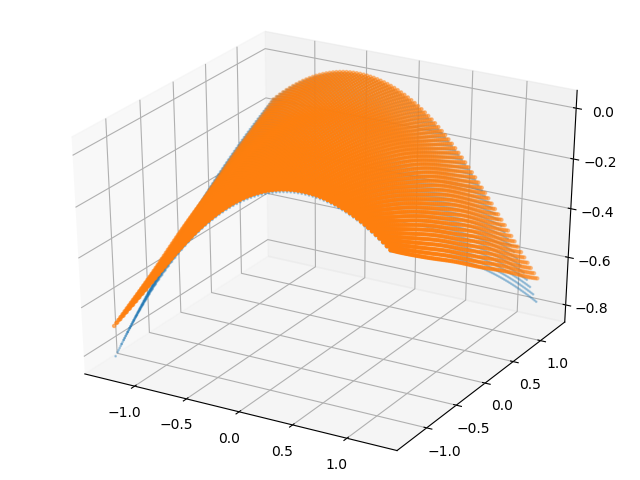
\includegraphics[width=\textwidth]{orig/Parabola-2D-_1D_BORING.png}
        \caption{Parabolanusoidal Boring}
        \label{fig:tiger}
    \end{subfigure}
     %add desired spacing between images, e. g. ~, \quad, \qquad, \hfill etc. 
    %(or a blank line to force the subfigure onto a new line)
    \vskip\baselineskip
    \begin{subfigure}[b]{0.30\textwidth}
        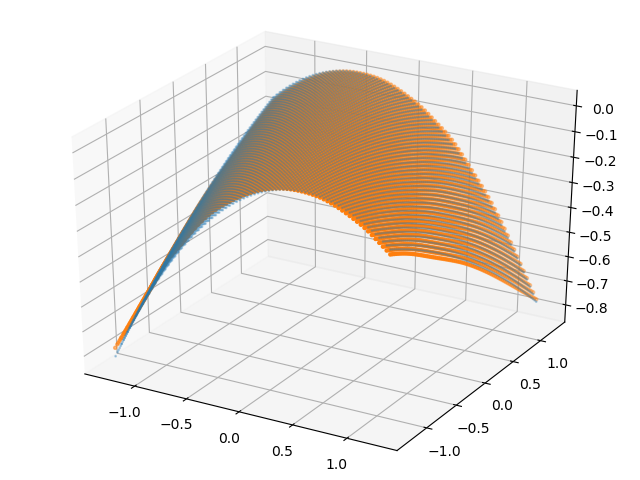
\includegraphics[width=\textwidth]{orig/Parabola-2D-_1D_TRIPATHY.png}
        \caption{Parabola Tripathy}
        \label{fig:mouse}
    \end{subfigure}
            %add desired spacing between images, e. g. ~, \quad, \qquad, \hfill etc. 
    %(or a blank line to force the subfigure onto a new line)
    \begin{subfigure}[b]{0.30\textwidth}
        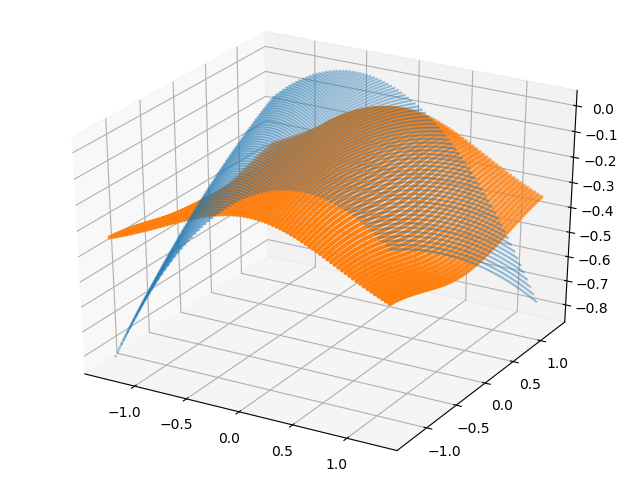
\includegraphics[width=\textwidth]{orig/Parabola-2D-_1D_REMBO.png}
        \caption{Parabola Rembo}
        \label{fig:mouse}
    \end{subfigure}
    \caption{Top-Left: The 1D Parabola which is embedded in a 2D space.}\label{fig:animals}
\end{figure}

I set the number of restarts to $14$ and number of randomly sampled data points to 100.
Notice that the Tripathy approximation is slightly more accurate than the BORING approximation. 
This is because one of Tripathy's initial starting points were selected better, such that algorithm 3 ran many times before the relative loss terminated the algorithm.
The active subspace projection matrix is of size $\mathbf{R}^{1 \times 2}$

% SINUSOIDAL FUNCTION
\begin{figure}[H]
    \centering
    \begin{subfigure}[b]{0.3\textwidth}
        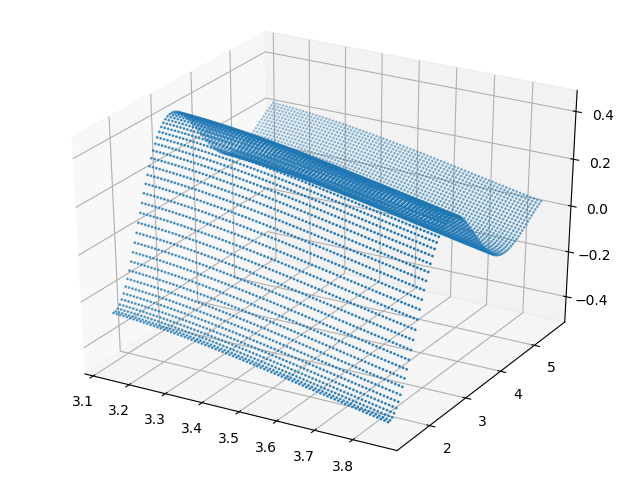
\includegraphics[width=\textwidth]{orig/Sinusoidal-5D-_2D.png}
        \caption{Sinusoidal Original}
        \label{fig:gull}
    \end{subfigure}
    ~ %add desired spacing between images, e. g. ~, \quad, \qquad, \hfill etc. 
      %(or a blank line to force the subfigure onto a new line)
    \begin{subfigure}[b]{0.3\textwidth}
        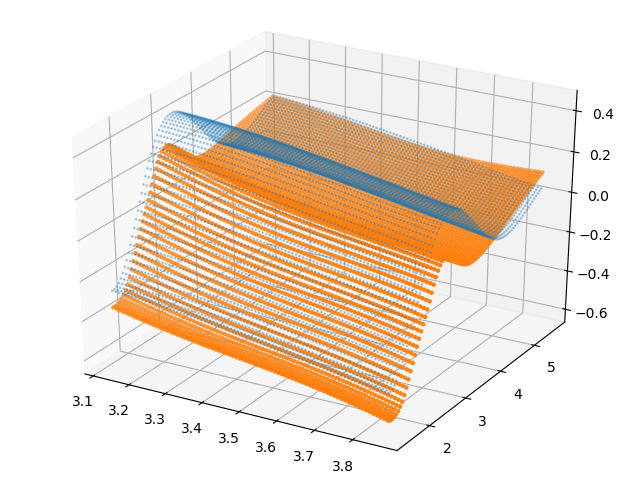
\includegraphics[width=\textwidth]{orig/Sinusoidal-5D-_2D_BORING.png}
        \caption{Sinusoidal Boring}
        \label{fig:tiger}
    \end{subfigure}
        \vskip\baselineskip
 %add desired spacing between images, e. g. ~, \quad, \qquad, \hfill, etc. 
    %(or a blank line to force the subfigure onto a new line)
    \begin{subfigure}[b]{0.3\textwidth}
        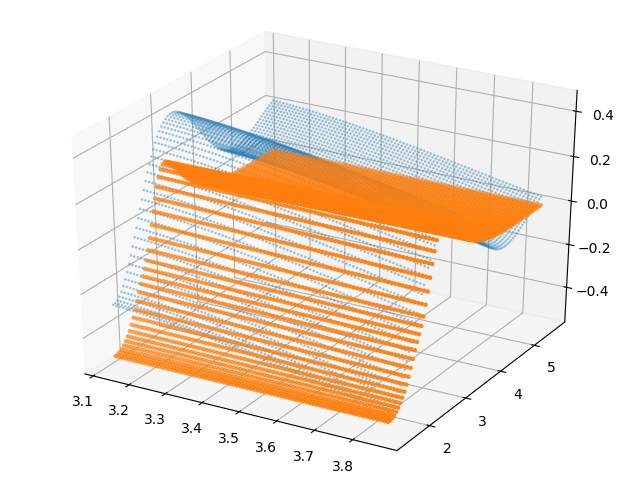
\includegraphics[width=\textwidth]{orig/Sinusoidal-5D-_2D_TRIPATHY.png}
        \caption{Sinusoidal Tripathy}
        \label{fig:mouse}
    \end{subfigure}
        ~ %add desired spacing between images, e. g. ~, \quad, \qquad, \hfill etc. 
    %(or a blank line to force the subfigure onto a new line)
    \begin{subfigure}[b]{0.3\textwidth}
        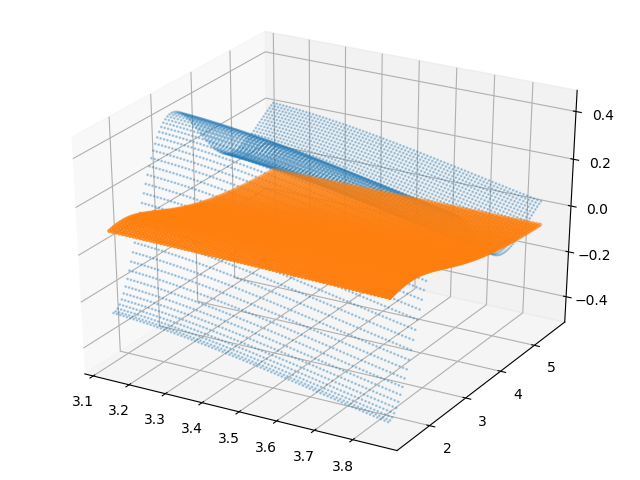
\includegraphics[width=\textwidth]{orig/Sinusoidal-5D-_2D_REMBO.png}
        \caption{Sinusoidal Rembo}
        \label{fig:mouse}
    \end{subfigure}
    \caption{Top-Left: The 2D Sinusoidal-Exponential Function which is embedded in a 5D space.}\label{fig:animals}
\end{figure}

I set the number of restarts to $28$ and number of randomly sampled data points to 100.
The active subspace projection matrix is of size $\mathbf{R}^{1\times 5}$, as this is a function that exhibits a strong principal component, but that still attains small perturbations among a different dimension.
One can see very well here, that BORING can take into account the small perturbations, at a considerably lower cost than Tripathy would be able to.


% CAMELBACK FUNCTION
\begin{figure}[H]
    \centering
    \begin{subfigure}[b]{0.3\textwidth}
        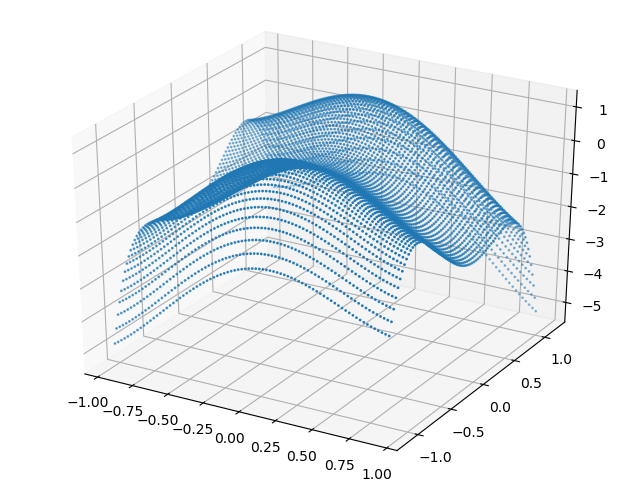
\includegraphics[width=\textwidth]{orig/Camelback-5D-_2D.png}
        \caption{Camelback Original}
        \label{fig:gull}
    \end{subfigure}
    ~ %add desired spacing between images, e. g. ~, \quad, \qquad, \hfill etc. 
      %(or a blank line to force the subfigure onto a new line)
    \begin{subfigure}[b]{0.3\textwidth}
        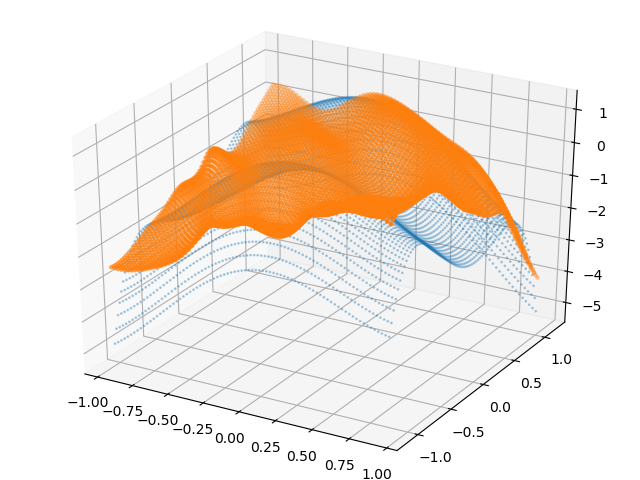
\includegraphics[width=\textwidth]{orig/Camelback-5D-_2D_BORING.png}
        \caption{Camelback Boring}
        \label{fig:tiger}
    \end{subfigure}
        \vskip\baselineskip
 %add desired spacing between images, e. g. ~, \quad, \qquad, \hfill, etc. 
    %(or a blank line to force the subfigure onto a new line)
    \begin{subfigure}[b]{0.3\textwidth}
        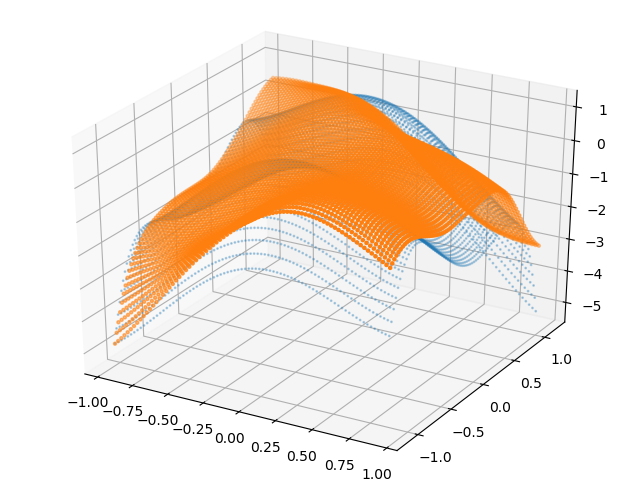
\includegraphics[width=\textwidth]{orig/Camelback-5D-_2D_TRIPATHY.png}
        \caption{Camelback Tripathy}
        \label{fig:mouse}
    \end{subfigure}
        ~ %add desired spacing between images, e. g. ~, \quad, \qquad, \hfill etc. 
    %(or a blank line to force the subfigure onto a new line)
    \begin{subfigure}[b]{0.3\textwidth}
        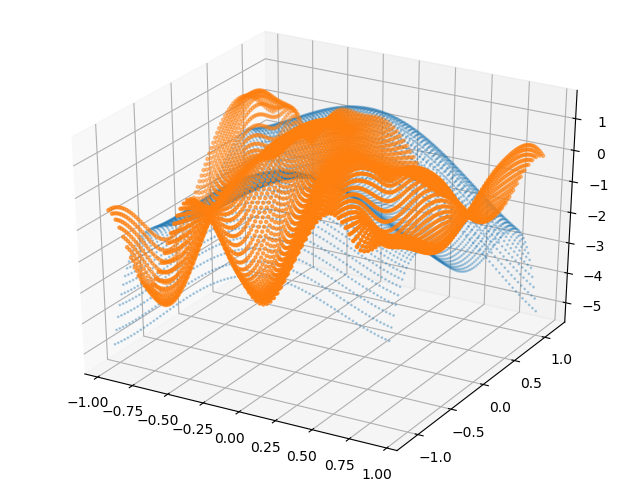
\includegraphics[width=\textwidth]{orig/Camelback-5D-_2D_REMBO.png}
        \caption{Camelback Rembo}
        \label{fig:mouse}
    \end{subfigure}
    \caption{Top-Left: The 2D Camelback Function which is embedded in a 5D space.}\label{fig:animals}
\end{figure}

I set the number of restarts to $28$ and number of randomly sampled data points to 100.
The active subspace projection matrix is of size $\mathbf{R}^{2 \times 5}$, as this is a function that lives in a 2D space, and has two strong principal components.
Notice that Tripathy and BORING use the same algorithm, as the visualization does not allow to add a third axis. 
In other words, BORING does not add any additional orthogonal vector to the model.
As such, it does not add any additional kernels to the model as well and is equivalent to Tripathy.
